\lhead{\begin{tikzpicture}[remember picture, overlay]
    \node [anchor=100,inner sep=0] (imagenIZQUIERDA) at (current page header area.north){
\includegraphics[width=18cm]{img/Encabezado.PNG}};
    \end{tikzpicture}}
    \rhead{Autor: primerApellido-segundoApellido}
    \rfoot{\begin{tikzpicture}[remember picture, overlay]
    \node [anchor=140,inner sep=0] (imagenDERECHA) at (current page footer area.south){
\includegraphics[width=18cm]{img/Foot.PNG}};
    \end{tikzpicture}}
    %----------------------------------------------------------------------------------------
    \lfoot{ \thepage}
    % \renewcommand{\labelenumi}{\alph{enumi}.)} 
    %----------------------------------------------------------------------------------------
    %----------------------------------------------------------------------------------------
    %	TITLE SECTION
    %----------------------------------------------------------------------------------------
    
    \setlength{\droptitle}{-5\baselineskip} % Move the title up
    \title{\textbf{Proyecto}} % Article title
    
     \author{ 
     \textsc{Nombre del Autor : }\\ 
    %  Afiliación:
     \texttt{ Nombre del Departamento : } \\ 
     \texttt{Nombre de la Universidad : } \\ 
     \texttt{Ciudad y País :}\\ 
     \texttt{Correo : } 
     \and 
     \textsc{Collman Granados Joseph Iker}\\ 
    %  Afiliación:
     \texttt{ Estudio del Tabajo II } \\ 
     \texttt{Instituto Tecnologico De Queretaro } \\ 
     \texttt{Queretaro , Mexico }\\ 
     \texttt{joseiker1603@gmail.com} 
    }
    
    
    %----------------------------------------------------------------------------------------
    
    % \begin{document}
    
    % Print the title
    \maketitle
    \thispagestyle{fancy}
    
    %----------------------------------------------------------------------------------------
    %	ARTICLE CONTENTS
    %----------------------------------------------------------------------------------------
    
    % \section*{Resumen}
    % \textit{Palabras clave:}
    % El resumen (ancho de página) deberá contener entre 100 y 200 palabras tipo Adobe Devangari 11 puntos.
    
    \begin{abstract}
    \noindent 
    Como un breve resumen lo que se busca es que el usuario entienda y comprenda lo que el potenciómetro  significa y cual es su uso que debe de ser correctamente el correcto para un mejor manera y esto haga que sea eficaz para el usuario y para la empresa el cual invierte en el producto para una mejora continua , esto hará que la comprensión del potenciómetro  sea el correcto y de una buena manera sobretodo para el aprendizaje y comprensión del proyecto
    
    \end{abstract}
    % 
    % 
    \textbf{\textit{Palabras clave}}: Ser exacto y Preciso .
    
    \section{Introducción}
    
    Para empezar con la  introducción tenemos que definir las piezas que vas a utilizar durante nuestro proceso el cual es el LCD , potenciómetro  , el SP32 
    , Cable macho-macho , cable macho-hembra , las resistencias , la interfaz de conexión l2c para la lcd , el cable usb , protobard y la resistencia de la luz , todos estos elementos son los que vamos a utilizar y vamos a emplear a cabo en cada etapa los cuales primero debemos de analizar y entender para darle su uso de debida forma .
    \newline
    
    % 
    %
    
    \textbf{\textit{1-El LCD }}: Es una pantalla de cristal liquido nombrada en sus siglas en ingles (LCD) que se utiliza para ver Imágenes fijas y en movimientos que va a estar formada por gran cantidad de pixel que consisten en Molécula s de cristal liquido contenidas entre dos conjuntos electrodos transparentes .
    \newline
     
    % 
    % 
    \textbf{\textit{1-El potenciometro }}: Es un dispositivo electrónico que nos va a ayudar de una manera exponencial ya que posee la resistencia
    variable Mecánica y sirve para controlar  el valor de la resistencia en vez de ser fijo es variable. 
    \newline
    
    % 
    % 
    \textbf{\textit{3-El SP32 }}: Aparte de integrar la radio  inalámbrica , sino también un procesador integrado con interfaces para conectarse con varios periférico  y controla otras cosas de mayor importancia .  
    \newline
    
    % 
    % 
    \textbf{\textit{4- Cable Macho-Macho  }}: se va a utilizar en el tablero protoboard haciendo posible la conexión de dos elementos ingresados en dichos tableros y se conoce así por los fragmentos que sobresalen de los extremos del cable .   
    \newline
    
    % 
    % 
    \textbf{\textit{5- Cable Macho-Hembra }}: a hembra se refiere a un conector que forma un tipo de manguito alrededor de su homologo masculino en el centro  ya que la hembra va a tener la rosca por dentro.
    \newline
    
    % 
    % 
    \textbf{\textit{6- Resistencias  }}: Estas están hechas de materiales que resisten el flujo de electricidad cuando pasa a través de ellas de esta manera se puede controlar el flujo de la corriente a través de un circuito .   \newline 
    
    % 
    % 
    \textbf{\textit{7- La interfaz de conexión l2c para la LCD  }}:  el modulo serial l2c permite manejar tu pantalla lcd de una manera bastante fácil esto permite enviar y recibir información y 2 mas para alimentación . \newline 
    
    % 
    % 
    \textbf{\textit{8-Cable USB }}: Definiremos como un conector que permite vincular una amplia variedad de elementos a través del universal serial bus . 
    \newline 
    
    % 
    % 
    \textbf{\textit{9- protoboard }}: se usa en proyectos de Robótica que permite conectar fácilmente componentes electrónicos entre si , sin necesidad de realizar una soldadura . 
    \newline 
    
    % 
    % 
    \textbf{\textit{10- conector base de luz  }}: sirve para que al conectar esa base nosotros tengamos energía directamente a  través  de una base y de su conector . 
    \newline
    
    \section { Objetivos }
    
    Uno de los principales objetivos es el que nosotros como usuario identifiquemos todas las etapas que va a tener desde la fase inicial hasta la fase final y también que el usuario conozca todo en lo engloba el proyecto para que así se pueda tener un mejor conocimiento para que al momento final se tenga de mejor manera uno de los principales objetivos es identificar , analizar , comprender y ejecutar .
    
    \section{Objetivos Específicos }
    
    Claro, basándome en la información proporcionada, aquí tienes algunos objetivos específicos que podrías considerar:
    
    1. Identificación clara de etapas del proyecto: Establecer claramente las diferentes etapas que componen el proyecto, desde la fase inicial hasta la fase final, para que los usuarios puedan entender la secuencia de actividades. 
    \newline
    
    2. Comunicación efectiva de los objetivos del proyecto: Asegurarse de que los usuarios comprendan los objetivos generales del proyecto, así como los beneficios que se esperan obtener al completarlo.
    \newline
    
    3. Detallar los componentes del proyecto: Proporcionar información detallada sobre todos los aspectos del proyecto, incluidos recursos necesarios, plazos, roles y responsabilidades, para que los usuarios tengan una comprensión completa de lo que implica participar en él. \newline
    
    4. Facilitar la comprensión del proceso: Desglosar cada etapa del proyecto en tareas específicas y acciones concretas, de modo que los usuarios puedan comprender fácilmente qué se espera de ellos en cada fase. 
    \newline
    
    5. Fomentar la participación activa de los usuarios: Establecer mecanismos para que los usuarios puedan involucrarse activamente en el proyecto, ya sea proporcionando retroalimentación, contribuyendo con ideas o participando en decisiones clave. 
    \newline
    
    6. Medir el progreso y el cumplimiento de hitos: Establecer indicadores claros para evaluar el progreso del proyecto y asegurarse de que se cumplan los hitos importantes en cada etapa. 
    \newline
    
    7. Evaluar y ajustar continuamente: Establecer un proceso para evaluar regularmente el progreso del proyecto, identificar áreas de mejora y realizar ajustes según sea necesario para garantizar el éxito final. \newline
    
    Estos objetivos específicos pueden ayudar a garantizar que los usuarios comprendan completamente el proyecto y estén equipados para contribuir de manera efectiva a su realización.
    
    \section{Descripción del Problema }
    El desafío del estudio de tiempos y movimientos en el ensamblaje de circuitos electrónicos implica una serie de complicaciones que pueden impactar tanto en la eficacia operativa como en la calidad del producto final. En resumen, este problema abarca diversos retos que afectan la eficiencia, calidad, seguridad laboral y rentabilidad del proceso de ensamblaje. Es crucial aplicar distintos métodos de optimización para abordar estos desafíos de manera efectiva y así fomentar la excelencia en la producción de circuitos electrónicos.
    
    \section{  Fundamentación teórica  }
    La base teórica del estudio de tiempos y movimientos en el ensamblaje de circuitos electrónicos se apoya en varios principios clave de la ingeniería industrial y la gestión de operaciones. Aquí tienes una descripción simplificada de algunos de estos conceptos:
    \newline
    
    1. Análisis de tiempos: Consiste en medir y registrar cuánto tiempo toma completar cada tarea individual en el proceso de ensamblaje. Esto ayuda a entender cómo se distribuye el tiempo entre diferentes actividades, lo que permite identificar oportunidades de mejora y eliminar tareas innecesarias o repetitivas. Este análisis proporciona una forma cuantitativa de evaluar la eficiencia del proceso y diseñar mejoras.
    \newline
    
    2. Cronometraje de movimientos: Se enfoca en analizar y mejorar los movimientos físicos realizados por los trabajadores durante el ensamblaje. Utiliza principios de ergonomía y biomecánica para identificar movimientos ineficientes o que puedan causar fatiga o lesiones. Optimizar estos movimientos puede mejorar la eficiencia del proceso y reducir el riesgo de lesiones laborales.
    \newline
    
    3. Estudio de métodos: Implica analizar y comparar diferentes métodos o técnicas utilizadas para realizar una tarea específica en el ensamblaje de circuitos electrónicos. El objetivo es encontrar el método más eficiente que permita completar la tarea de manera rápida, precisa y segura. Esto puede incluir la evaluación de herramientas, equipos, diseños de estaciones de trabajo y procedimientos de trabajo.
    
    \section{Justificación }
    El análisis de tiempos y movimientos en la producción de circuitos electrónicos es esencial debido a diversos factores críticos que influyen tanto en la eficacia operativa como en la calidad del producto terminado. A continuación, se exponen algunas razones que respaldan la importancia de realizar este análisis utilizando diversas estrategias para mejorar la eficiencia.
    \newline
    
    Eficiente utilización de recursos: La producción de circuitos electrónicos requiere una gestión precisa de los recursos disponibles, como el tiempo, la mano de obra y los materiales. Optimizar estos aspectos mediante el análisis de tiempos y movimientos garantiza un uso más efectivo de los recursos disponibles, lo que puede conducir a una reducción de costos y un aumento en la productividad.\newline
    
    El análisis de tiempos y movimientos en la producción de circuitos electrónicos es crucial debido a varios factores críticos que impactan tanto en la eficacia operativa como en la calidad del producto final. Aquí hay una ampliación sobre la importancia de este análisis: \newline
    
    1. Eficiente utilización de recursos: La producción de circuitos electrónicos implica la gestión precisa de recursos como el tiempo, la mano de obra y los materiales. El análisis de tiempos y movimientos permite identificar áreas donde se puede optimizar el uso de estos recursos. Por ejemplo, al reducir el tiempo dedicado a ciertas tareas o minimizar los movimientos innecesarios de los trabajadores, se puede mejorar la eficiencia general del proceso. Esta optimización conduce a una mejor utilización de los recursos disponibles, lo que puede resultar en una reducción de costos y un aumento de la productividad. \newline
    
    2. Mejora en la planificación y programación: Conocer el tiempo necesario para completar cada tarea en el proceso de producción de circuitos electrónicos facilita una mejor planificación y programación de la producción. Al tener datos precisos sobre los tiempos de ciclo, es posible establecer cronogramas realistas y evitar retrasos en la entrega de productos. Además, permite una asignación más eficiente de la mano de obra y los recursos, evitando la subutilización o sobreutilización de los mismos. \newline
    
    3. Identificación de cuellos de botella y áreas de mejora: El análisis de tiempos y movimientos revela cuellos de botella y áreas de ineficiencia en el proceso de producción. Identificar estos puntos críticos permite tomar medidas correctivas para mejorar la fluidez del proceso y aumentar la capacidad de producción. Por ejemplo, si se descubre que una máquina específica está causando retrasos recurrentes, se pueden implementar medidas para optimizar su funcionamiento o considerar la inversión en equipos más eficientes.\newline
    
    4. Aumento de la calidad del producto: Al optimizar los tiempos y movimientos en la producción de circuitos electrónicos, se reduce la probabilidad de errores y defectos en el producto final. Los procesos más eficientes tienden a ser más consistentes y menos propensos a fallos, lo que se traduce en una mejora de la calidad del producto. Además, al minimizar los movimientos repetitivos y fatigantes para los trabajadores, se reduce el riesgo de errores humanos y se mejora la precisión en el ensamblaje. \newline
    
    En resumen, el análisis de tiempos y movimientos en la producción de circuitos electrónicos es esencial para optimizar el uso de recursos, mejorar la planificación y programación, identificar áreas de mejora y aumentar la calidad del producto final. Esto contribuye significativamente a la eficacia operativa y la competitividad de la empresa en el mercado.
    
    \section{  hipótesis }
    
    uno de los factores que puede ayudar de una mejor manera es la reducción de tiempos de ciclo el cual sugiere que al aplicar  técnicas de análisis de tiempos y movimientos, junto con métodos de optimización, se pueden reducir significativamente los tiempos necesarios para ensamblar circuitos electrónicos, lo que mejora la eficiencia del proceso.
    \newline
    
    otro factor sera la mejora de calidad de producto Se plantea que al optimizar los movimientos y métodos de ensamblaje, se pueden reducir los errores y defectos en los circuitos electrónicos ensamblados, lo que conduce a una mejora general en la calidad del producto final. \newline
    
    la mejora de Ergonomía y reducción de la fatiga  al analizar y optimizar los movimientos de los trabajadores durante el ensamblaje, se puede mejorar la ergonomía de las estaciones de trabajo, lo que reduce la fatiga y disminuye el riesgo de lesiones laborales , estos son factores que nos pueden ayudar de una mejor manera y tener en cuenta al momento de realizar el proyecto. \newline
    
    \subsection{ Análisis}
    Lo que se busca en estas etapas de comprensión de cómo se va a manejar el uso del dispositivo  y como se va a operar y claramente la función que va a tener para que así no tenga  alguna complicación,  esto se puede interpretar el análisis que va a tener el proyecto entiendo su armamento  desde el principio hasta el final , ahora lo que se debe de hacer es que
    
    \section{Cuerpo (Metodología, Pasos , etc.)}
    
    Aquí se va a describir las etapas que se hicieron para llegar al resultado final el cual fue nosotros hiciéramos un debido manejo de como se armará el proyecto hasta el final
    
    \section{Materiales )}
    
    -Regulador de voltaje 
    -USB 
    -protoboard 
    -ESP 
    -resistencias 
    -LCD 
    -modulo 
    -cable macho-macho 
    -cable macho-hembra 
    -almohadilla ,
    -potenciómetro 
    
    \subsection{Protoboard }
    
    Primero vamos a establecer como nuestra base el protoboard al cual vamos a conectar el SP32  y lo vamos a establecer fijo para conectarlo y soldarlo  , después al protoboard vamos a juntar los cables Macho - macho y el cable macho- hembra los cuales van a ser nuestros cables principales una vez teniendo eso lo que vamos a hacer es que vamos a conectar nuestro cable usb a una de las terminales del protoboard .
    \subsection{Cargador }
    Ese cable que seria nuestro cargador lo que va a hacer es que lo vamos a conectar a la base de luz para así empezar a tener energía  para que nuestro  puerto del protoboard empiece a funcionar debidamente  una vez teniendo esto plenamente  ahora nos vamos a enfocar en la pantalla .
    
    \subsection{LCD}
    
    Para continuar  vamos a tener la pantalla del Lcd y la vamos a soldar a la interfaz de conexión l2c para la lcd y así hacer que empiece a funcionar  una vez que el lCd esté funcionando eso va a querer significar que lo podemos conectar los cables macho - macho y el cable macho-hembra  a la pantalla para que esta valla indicando  el nivel de la energía que watts y nos va a decir nuestro nivel de voltaje que tenemos dependiendo de lo que el usuario manipule el divisor del potenciómetro . 
    
    \subsection{potenciómetro }
    Ahora nos vamos a enfocar en el potenciómetro  ya que esto va a hacer de vital importancia por que el usuario va a manipular al perilla que tiene el potenciómetro  para controlar el nivel de voltaje que va a tener , teniendo en cuenta  esto vamos a conectar el potenciómetro  al protoboard para que así pueda regular la energía de una mejor manera
    
    \begin{table} [H]
          
      \huge
      \tiny 
      \begin{tabular}   {| c |  c |  c | }
      
      \hline
      NOMBRE & imagen  & pieza \\
      \hline 
      potenciómetro  &  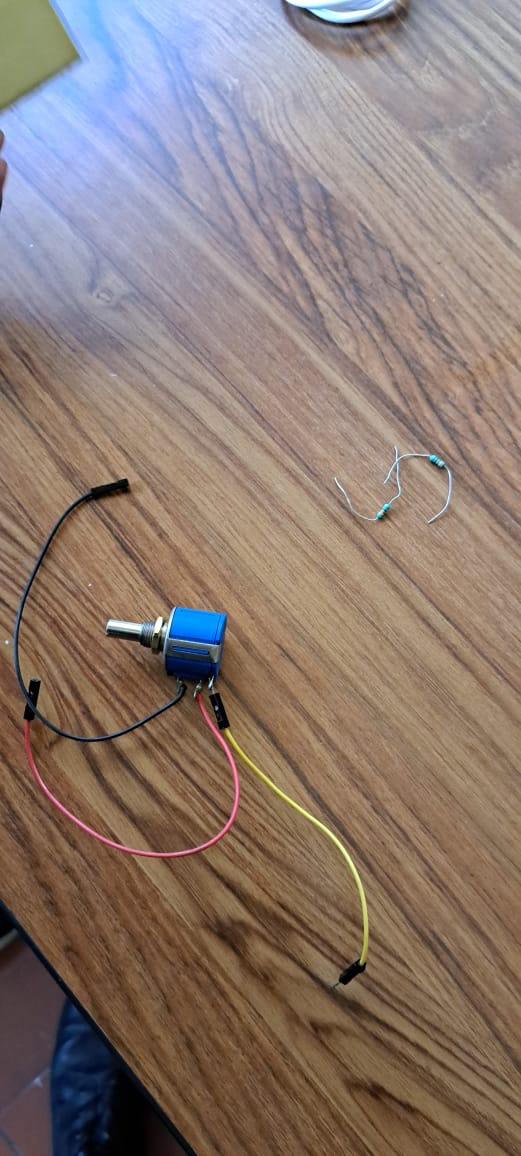
\includegraphics[height=19mm]{7/img/potenciometro.jpg}  & 
       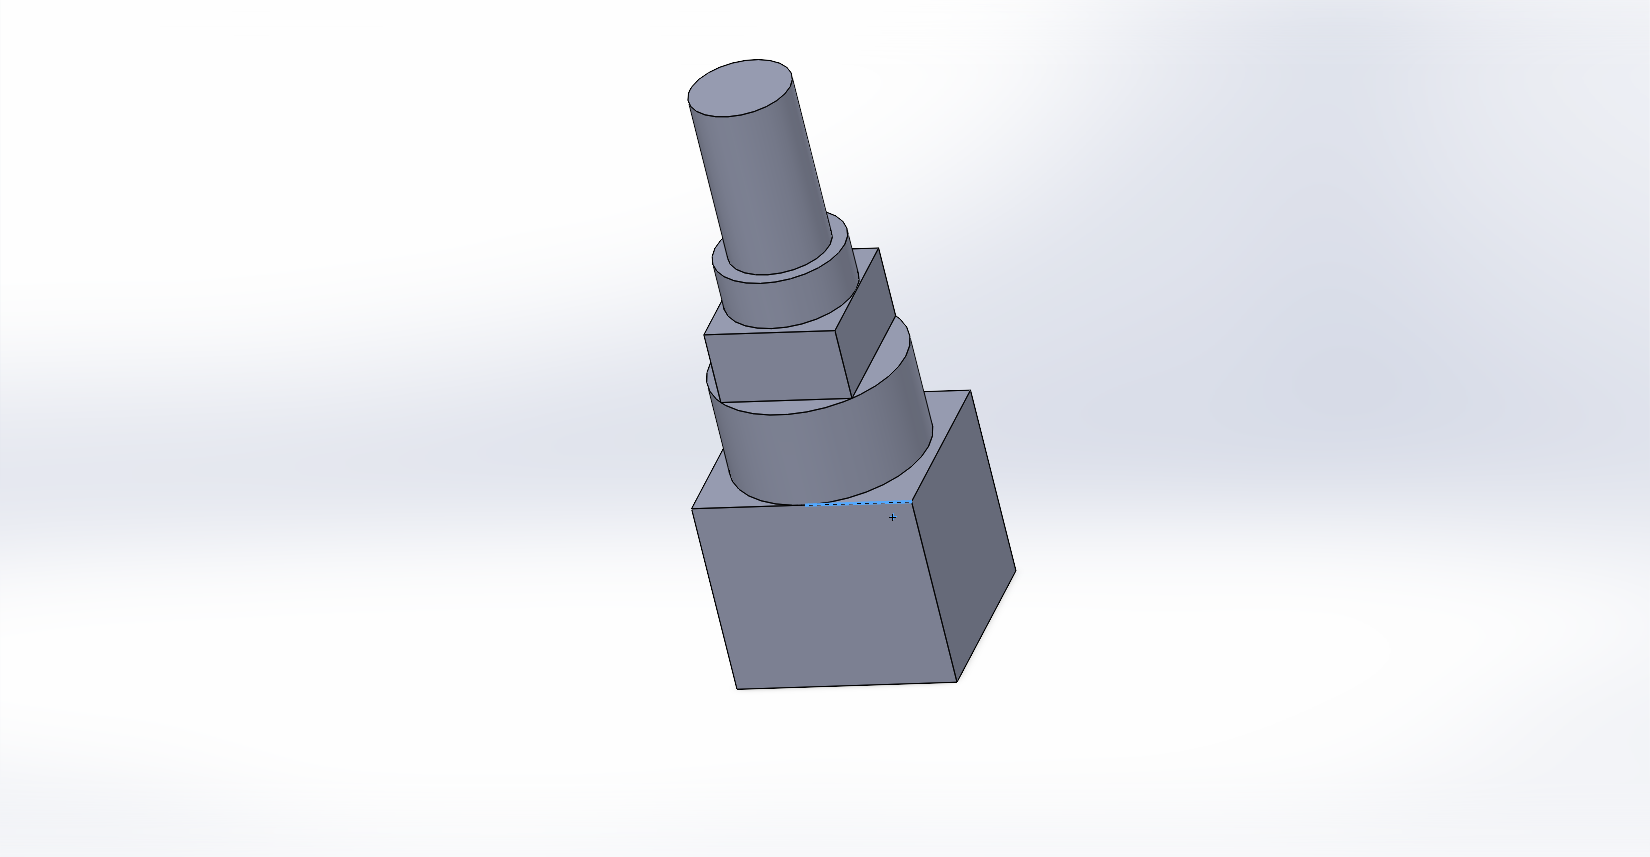
\includegraphics[width=19mm]{7/img/piezaaauno.PNG} \\
        \hline
      protoboard &  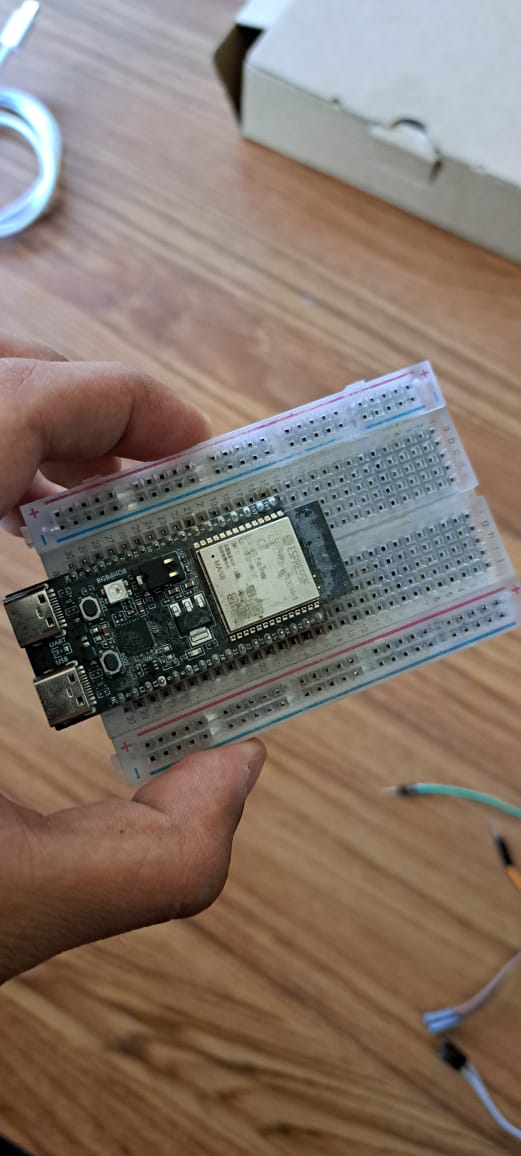
\includegraphics[height=19mm]{7/img/protoboard.jpg}  & 
       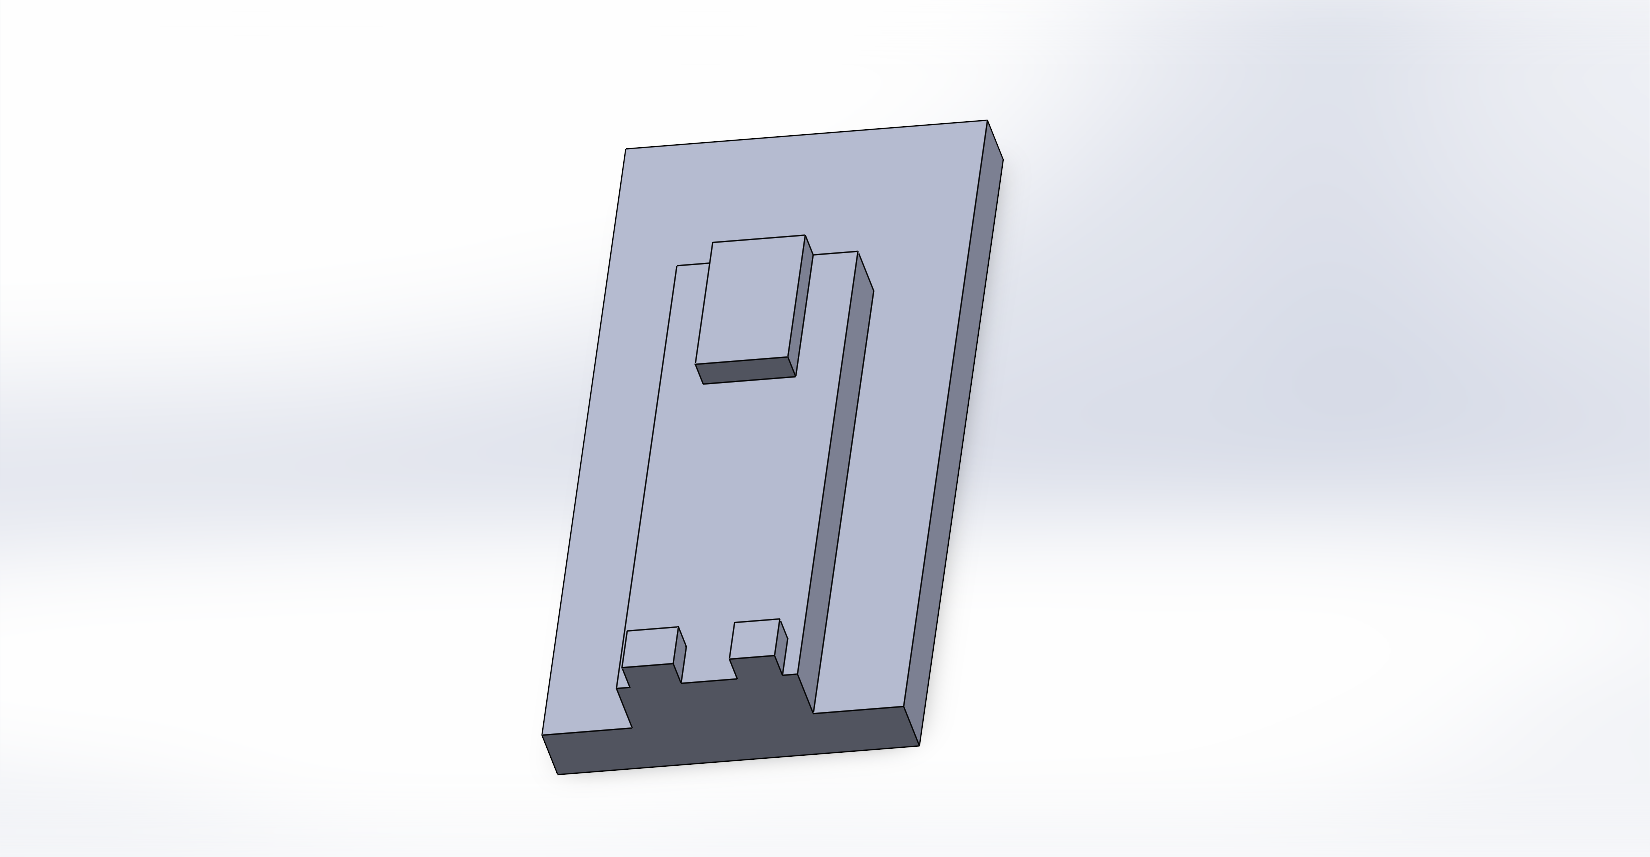
\includegraphics[width=19mm]{7/img/Piezauno.PNG} \\
        \hline
        lcd & 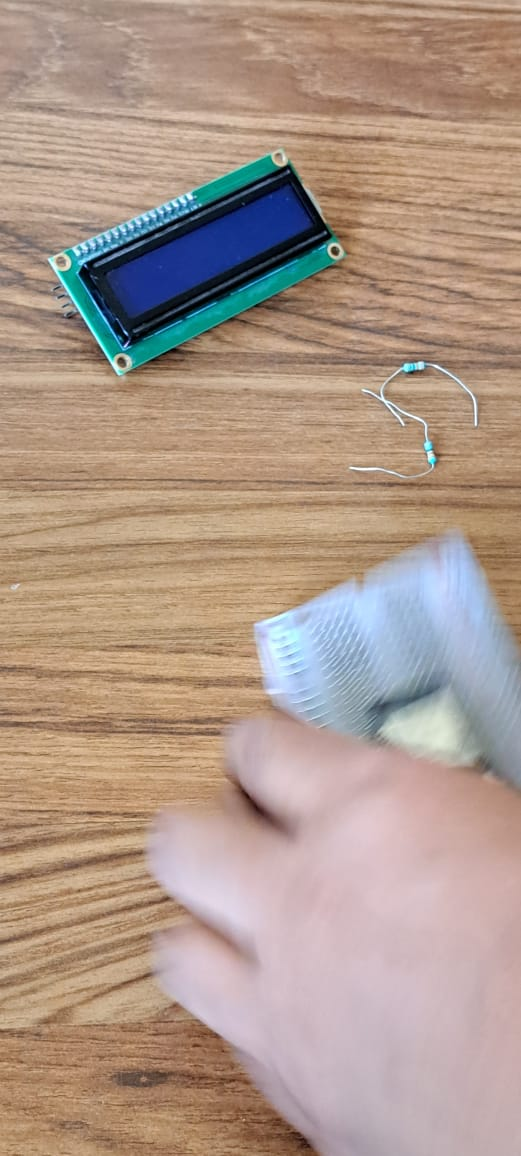
\includegraphics[height=19mm]{7/img/lcd.jpg}  & 
       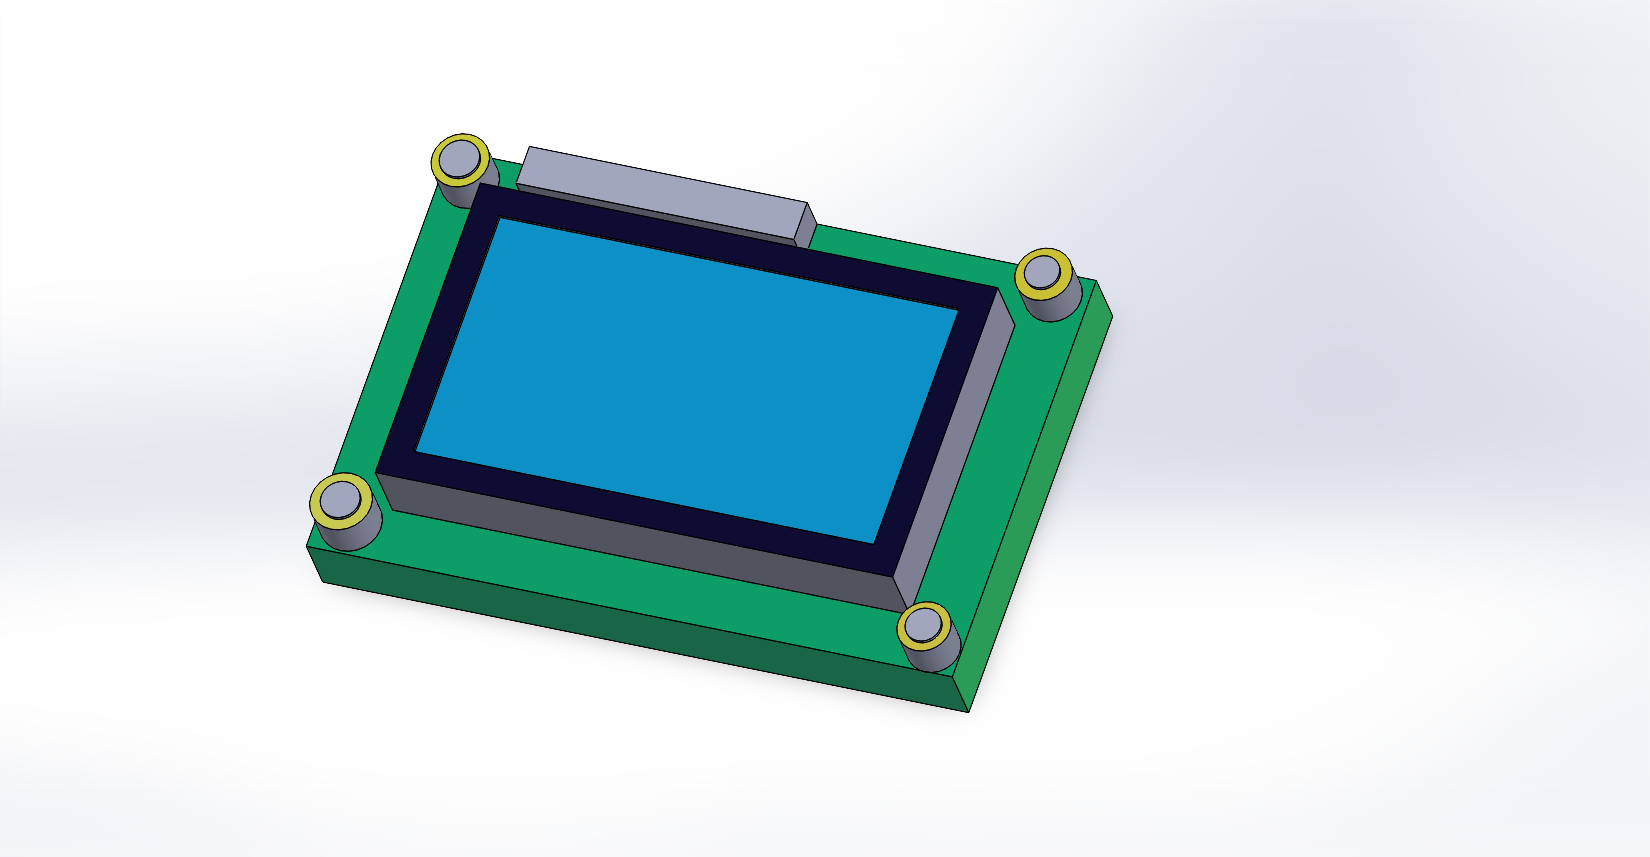
\includegraphics[width=19mm]{7/img/piezatress.PNG} \\
        \hline
        cable HM & 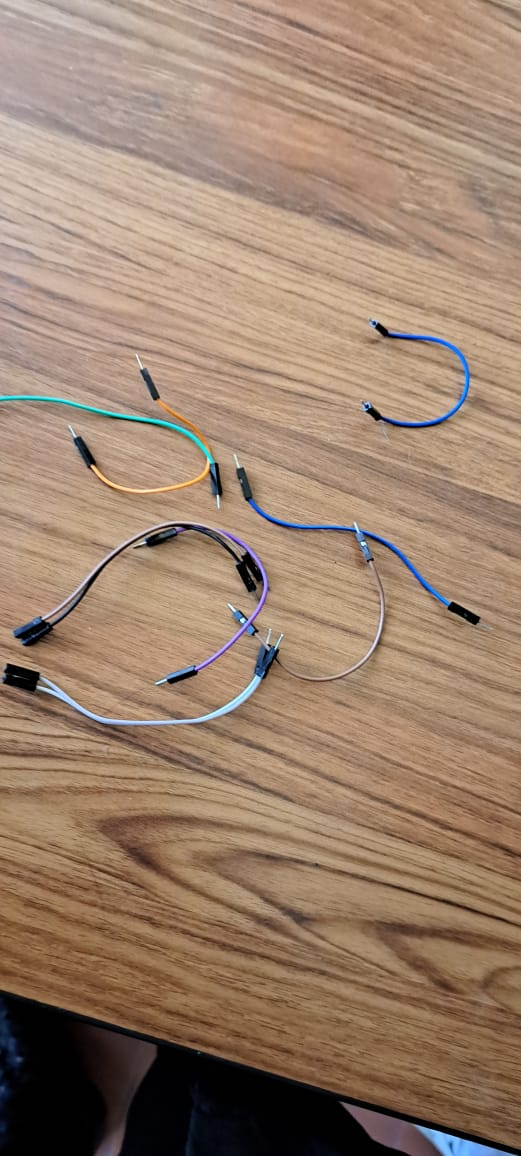
\includegraphics [height=19mm]{7/img/cables.jpg}  & 
       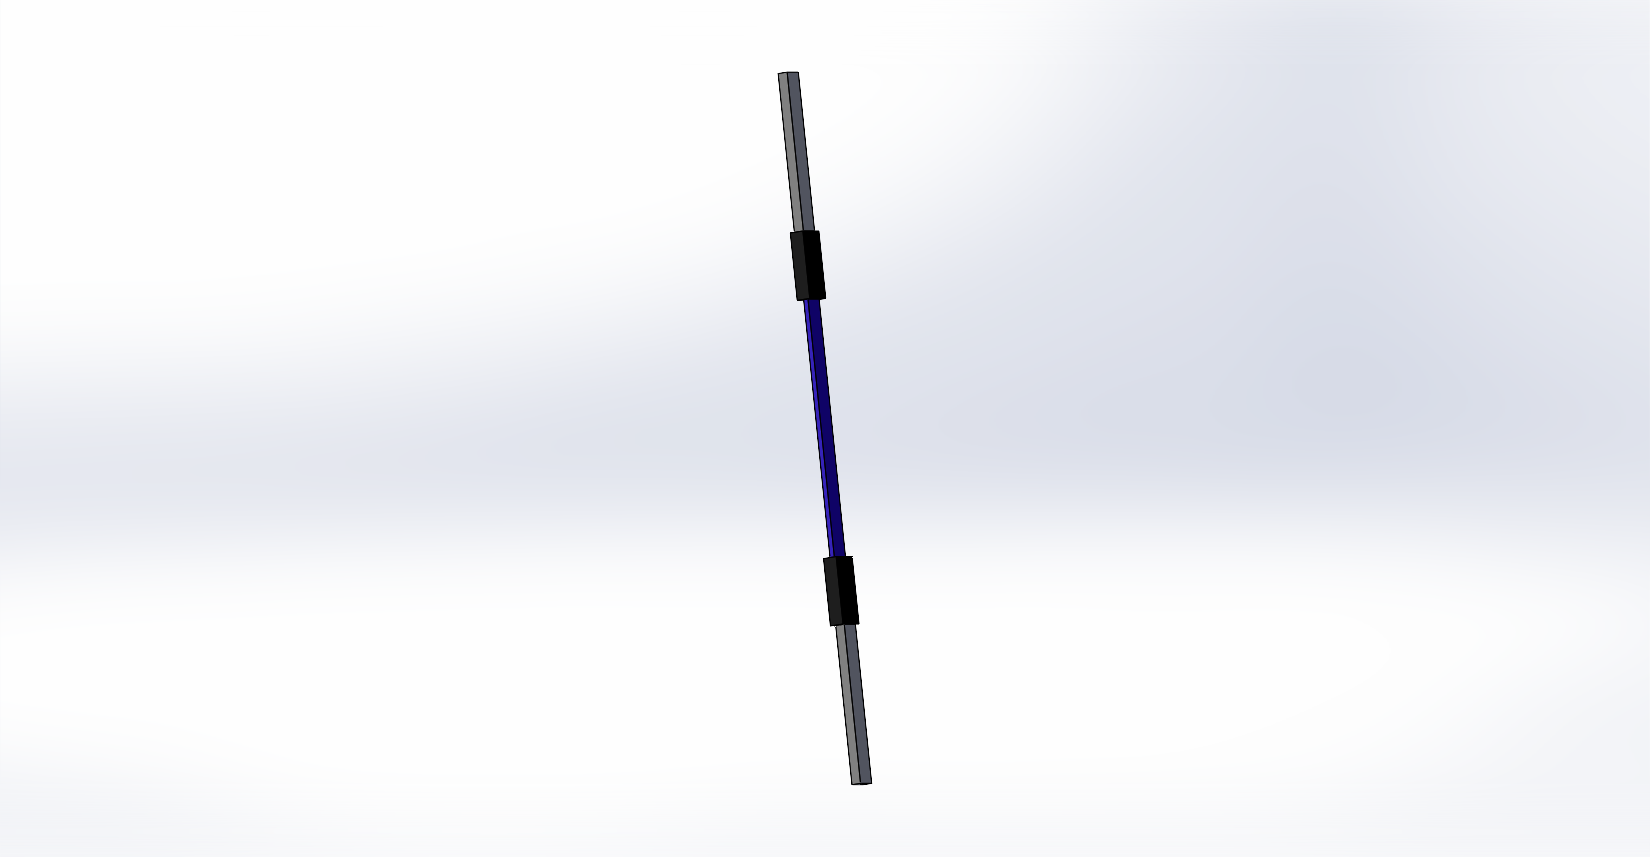
\includegraphics[width=19mm]{7/img/cuatrooo.PNG} \\
        \hline
        CABLE HH & 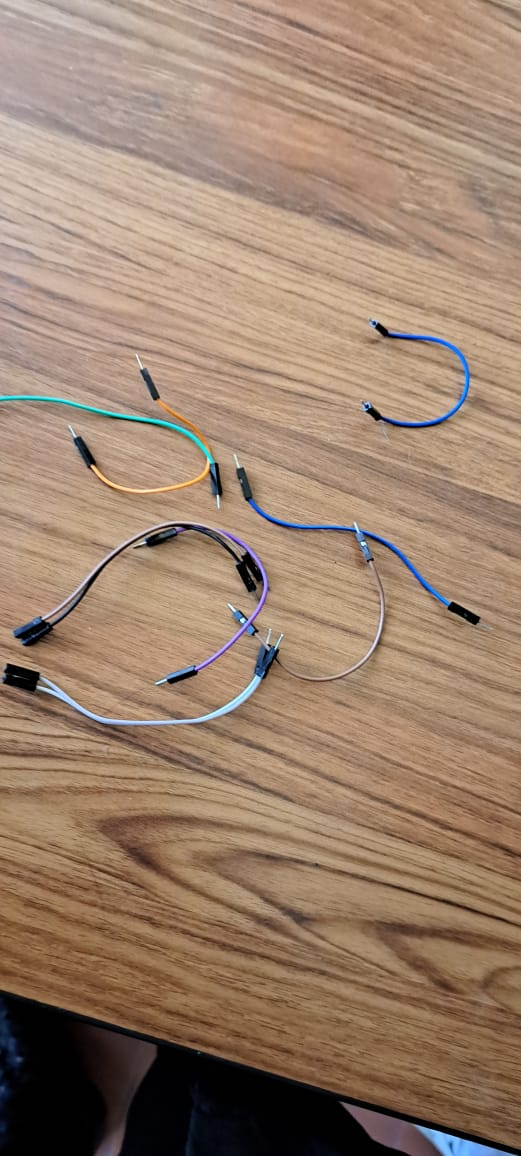
\includegraphics[height=19mm]{7/img/cables.jpg}  & 
       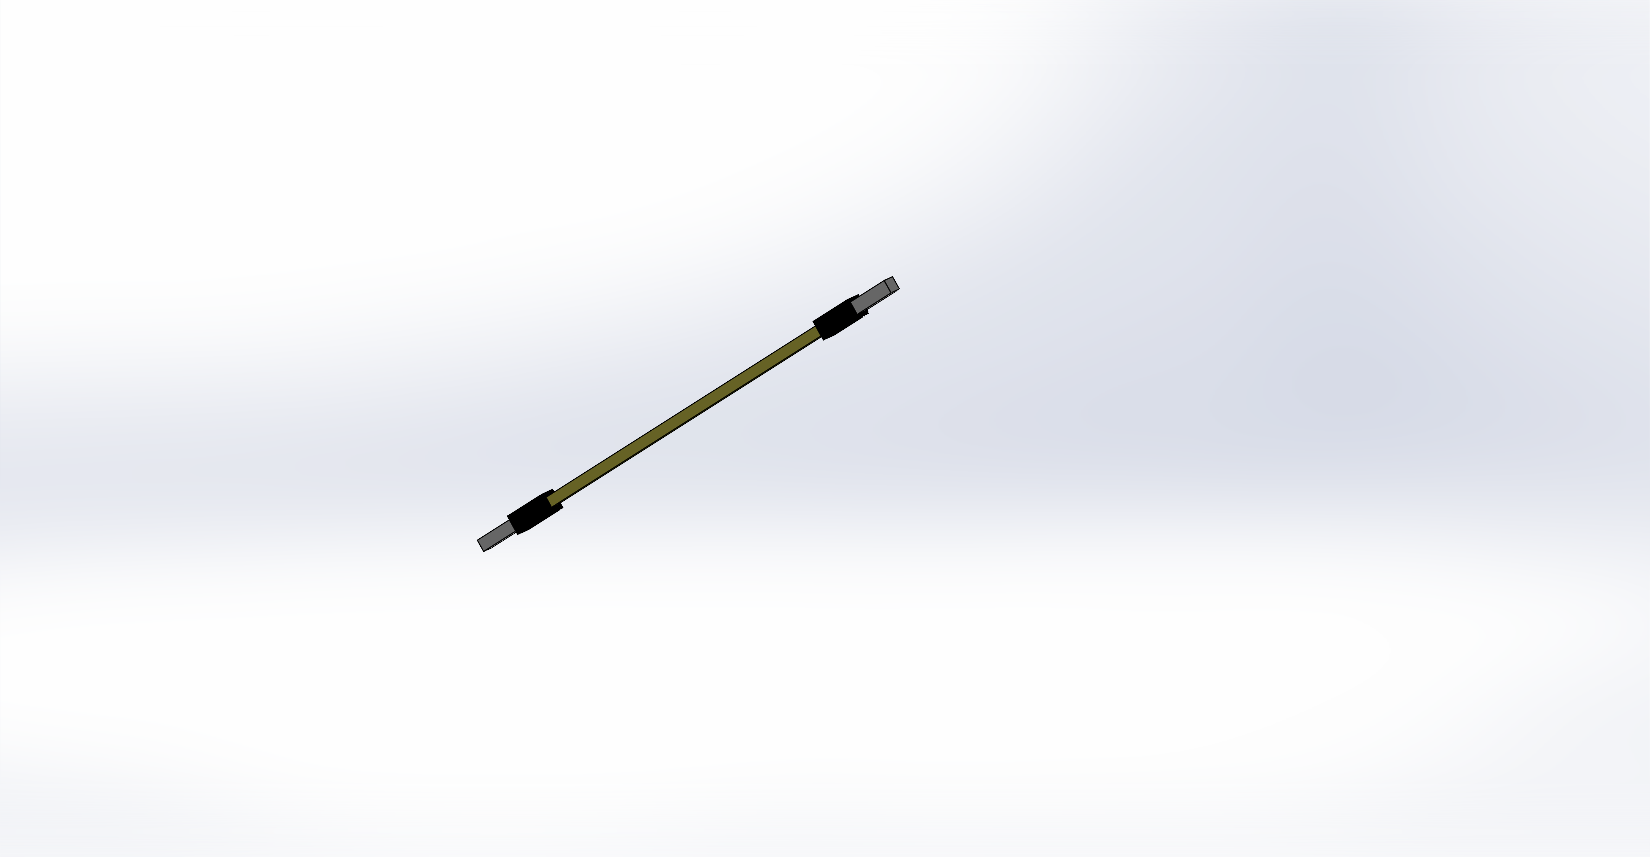
\includegraphics[width=19mm]{7/img/cinco.PNG} \\
        \hline 
         CABLE 1 & 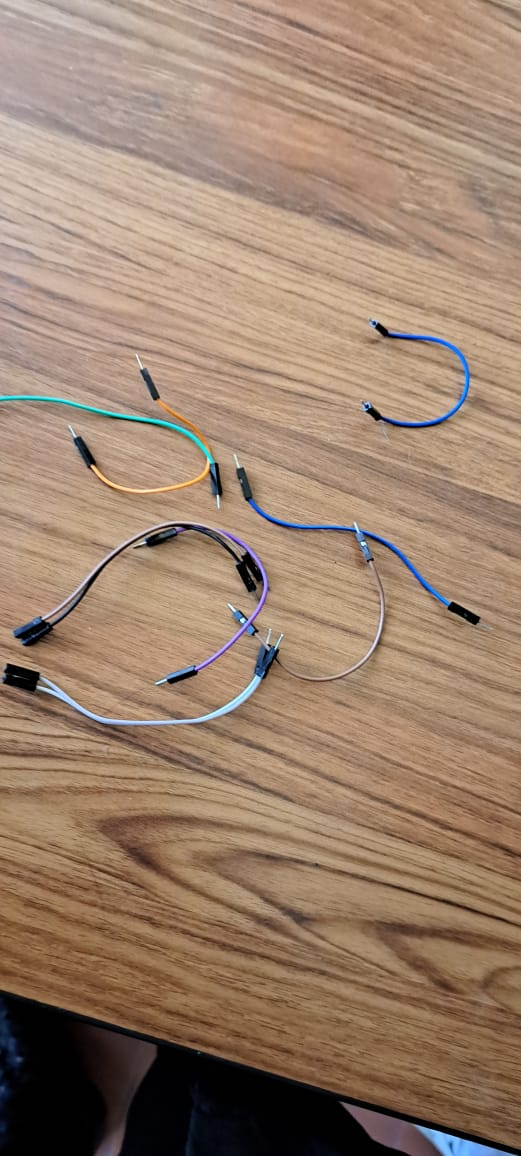
\includegraphics[height=19mm]{7/img/cables.jpg}  & 
       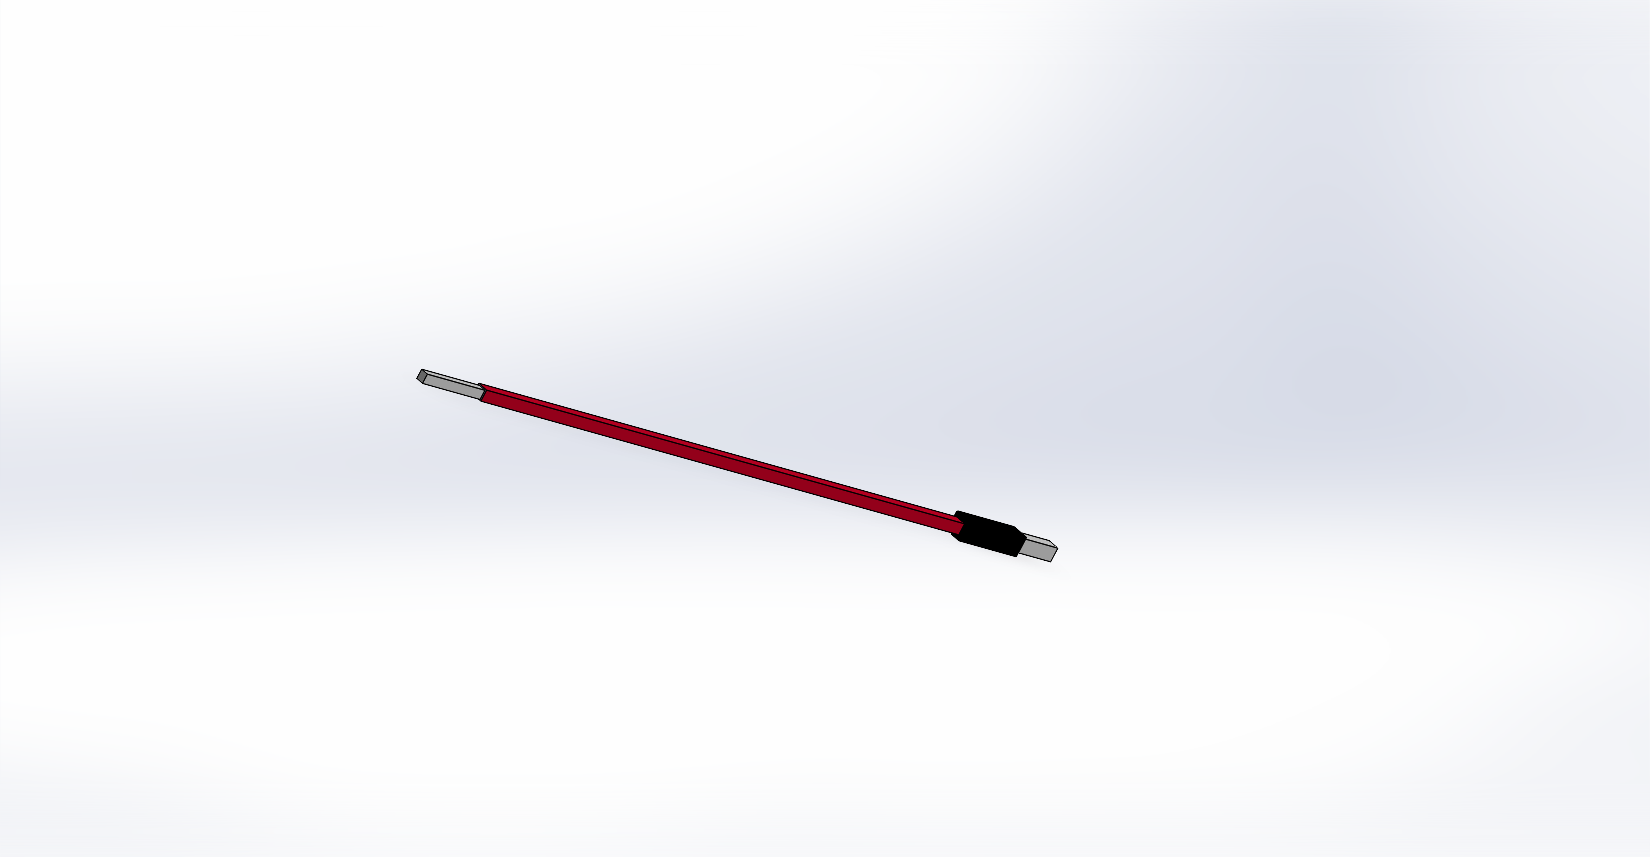
\includegraphics[width=19mm]{7/img/seis.PNG} \\
        \hline 
         CABLE 2 & 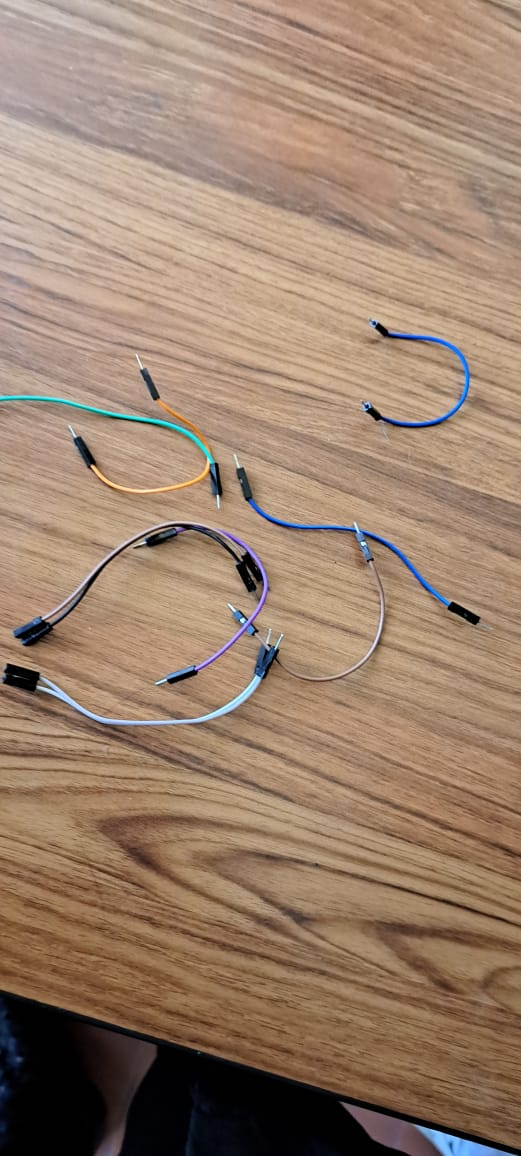
\includegraphics[height=19mm]{7/img/cables.jpg}  & 
       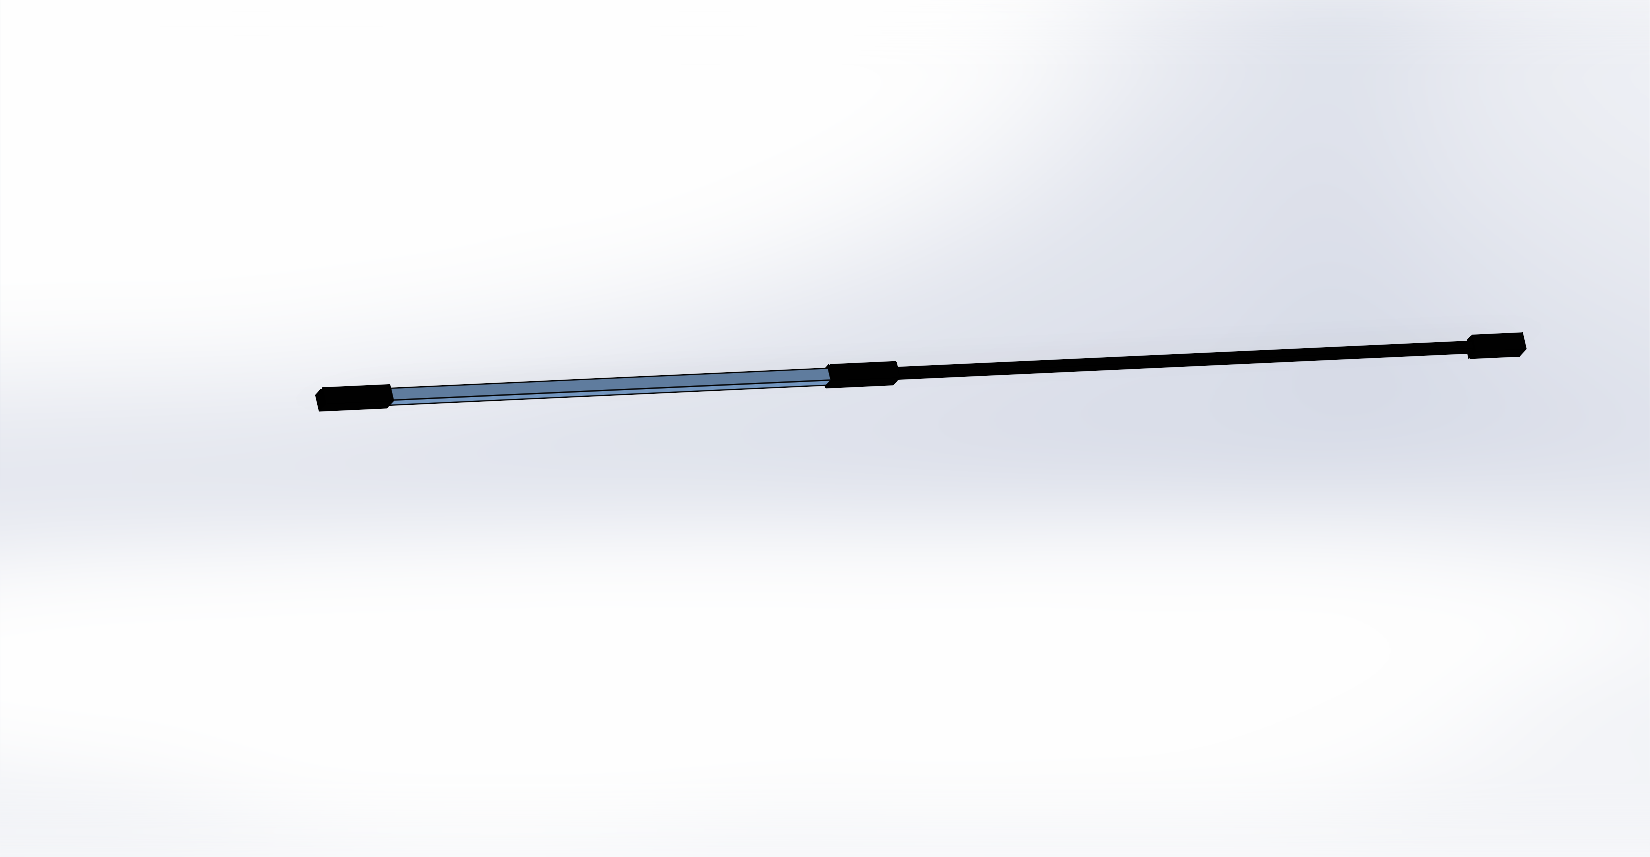
\includegraphics[width=19mm]{7/img/siete.PNG} \\
        \hline 
        
        \end{tabular} 
       
         \label {tab:my_label1}  \label {7/}
          \end{table} 
    
      \begin{tabular}{c|c}
           &  \\
           & 
      \end{tabular}  
    
    \subsection{Manual}
    
    \begin{table} [H]
          
      \huge
      \tiny 
      \begin{tabular}   {| c |  c |  c | }
      
     
     \hline 
      manual  &  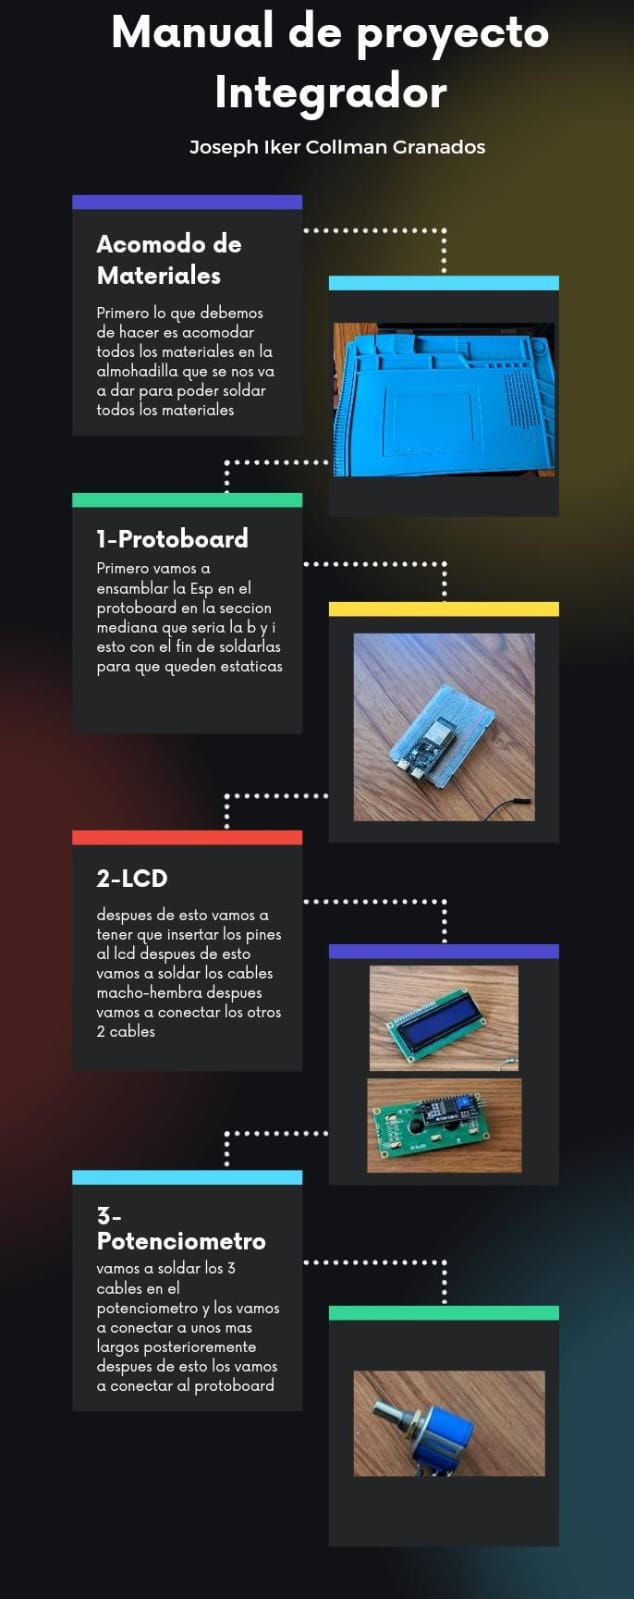
\includegraphics[height=90mm]{7/img/ikerv1.jpg}  & 
       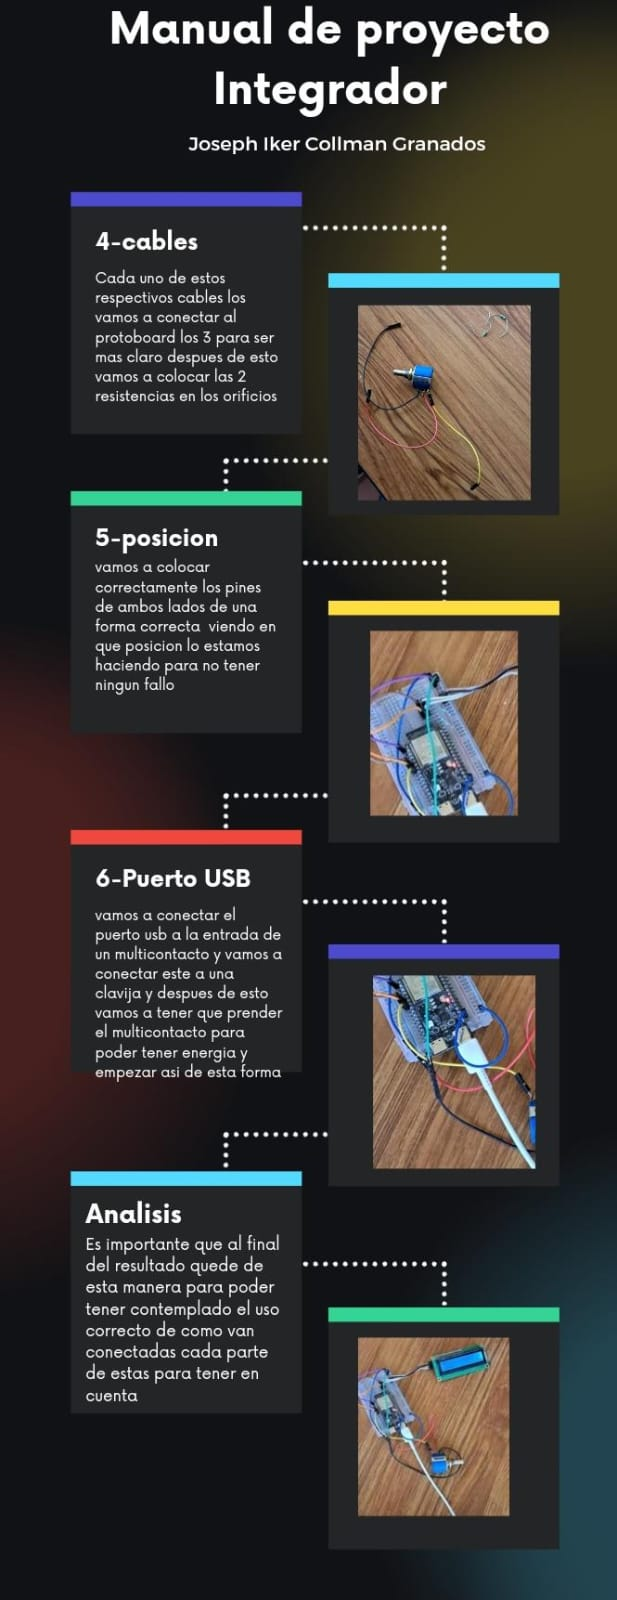
\includegraphics[width=35mm]{7/img/ikerv2.jpg} \\
        \hline
         
        \end{tabular} 
       
         \label {tab:my_label2}  \label {7/}
          \end{table} 
    
      \begin{tabular}{c|c}
           &  \\
           & 
      \end{tabular}  
        
    \subsection{Prepara tu documento}
    
        Antes de que comiences a utilizar esta plantilla, es recomendable que prepare la información que contendrá en un archivo aparte. 
        Ten preparadas tus gráficas, así como también las tablas aparte, para que sea más fácil integrarlo. 
        Se recomienda fuertemente el uso de \textbf{formato Enhanced Metafile (.emf) para imágenes y gráficas} de resolución óptima. 
        Finalmente, completa y organiza el contenido antes de darle el formato de esta plantilla. 
    
        \subsection{Acrónimos y Abreviaciones}
    
        Los acrónimos y abreviaciones deberán ser definidos únicamente la primera vez que aparecen en el texto, esto para que el lector entienda lo que significan.
    
        \subsection{Ecuaciones}
    
        Las ecuaciones son una excepción a las especificaciones prescritas de esta plantilla. 
        Deberá determinar si su ecuación debe escribirse o no utilizando la fuente Adobe Devangari. 
        Para crear ecuaciones multinivel, puede ser necesario tratar la ecuación como un gráfico e insertarla en el texto después de aplicar el estilo de la platilla.
        Las ecuaciones serán enumeradas de manera consecutiva, y el número de ecuación, entre paréntesis, se colocan al ras de la derecha, utilizando una tabulación derecha. 
    
        \begin{equation}
            \label{eq1}
            x + y = z 
        \end{equation}
    
        Es importante asegurarse de que los símbolos de la ecuación sean definidos antes o inmediatamente después de la ecuación. Utilice “(1)”, en vez de “Eq. 1” al enumerar las ecuaciones, excepto al principio de una oración: “La ecuación (\ref{eq1}) es…
    
        \subsection{Autores y Afiliaciones}
    
        Para distinguir las afiliaciones de los autores, utilice superíndices iniciando con el número 1, 2, etc., sucesivamente, esto dependerá de la cantidad de los departamentos a los que estén afiliados los autores. En caso de que todos los autores pertenezcan a una mismo departamento e institución, utilizar sólo el superíndice 1. 
    
        \subsection{Identificar los encabezados}
    
        Se les recuerda a los autores que los encabezados deben de estar conforme los solicita la guía del autor. De ahí se puede adaptar el trabajo para que sea más fácil de entender para el lector.
        Los encabezados organizan los temas sobre una base relacional y jerárquica. Por ejemplo, el título del documento es encabezado del texto principal porque todo el material posterior se relaciona y elabora sobre este tema.
        
    \subsection{Tablas y Figuras}
    
    \begin{table} [H]
          
      \huge
      \tiny 
      \begin{tabular}   {| c |  c |  c | }
      
      \hline
      NOMBRE & PIEZA  & PLANO \\
      \hline 
      potenciómetro  &  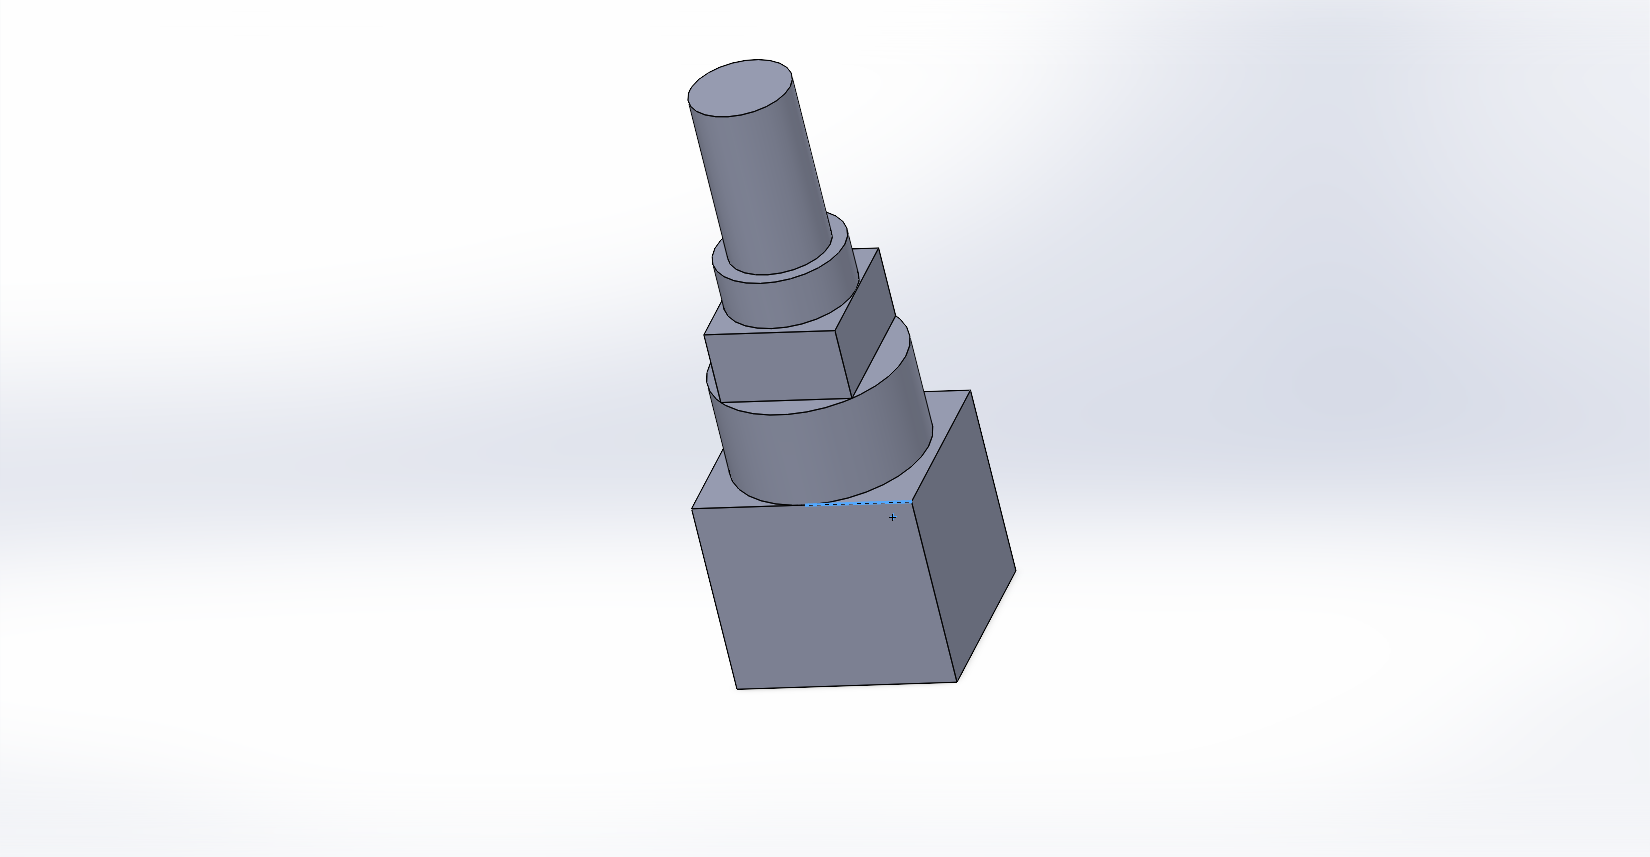
\includegraphics[height=19mm]{7/img/piezaaauno.PNG}  & 
       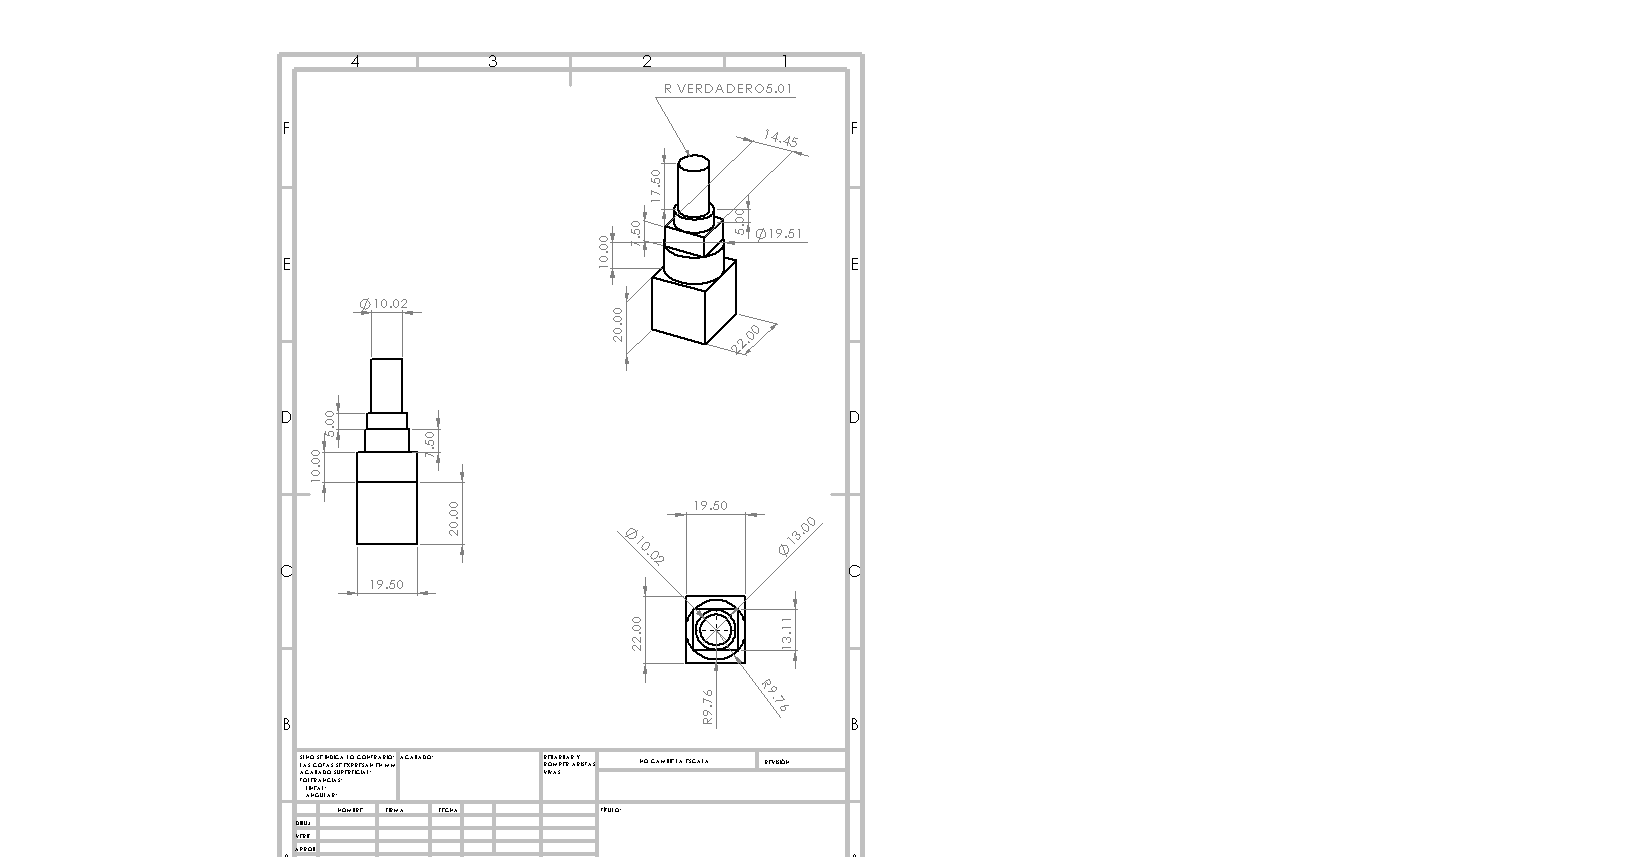
\includegraphics[width=19mm]{7/img/Pieza1.PNG} \\
        \hline
      protoboard &  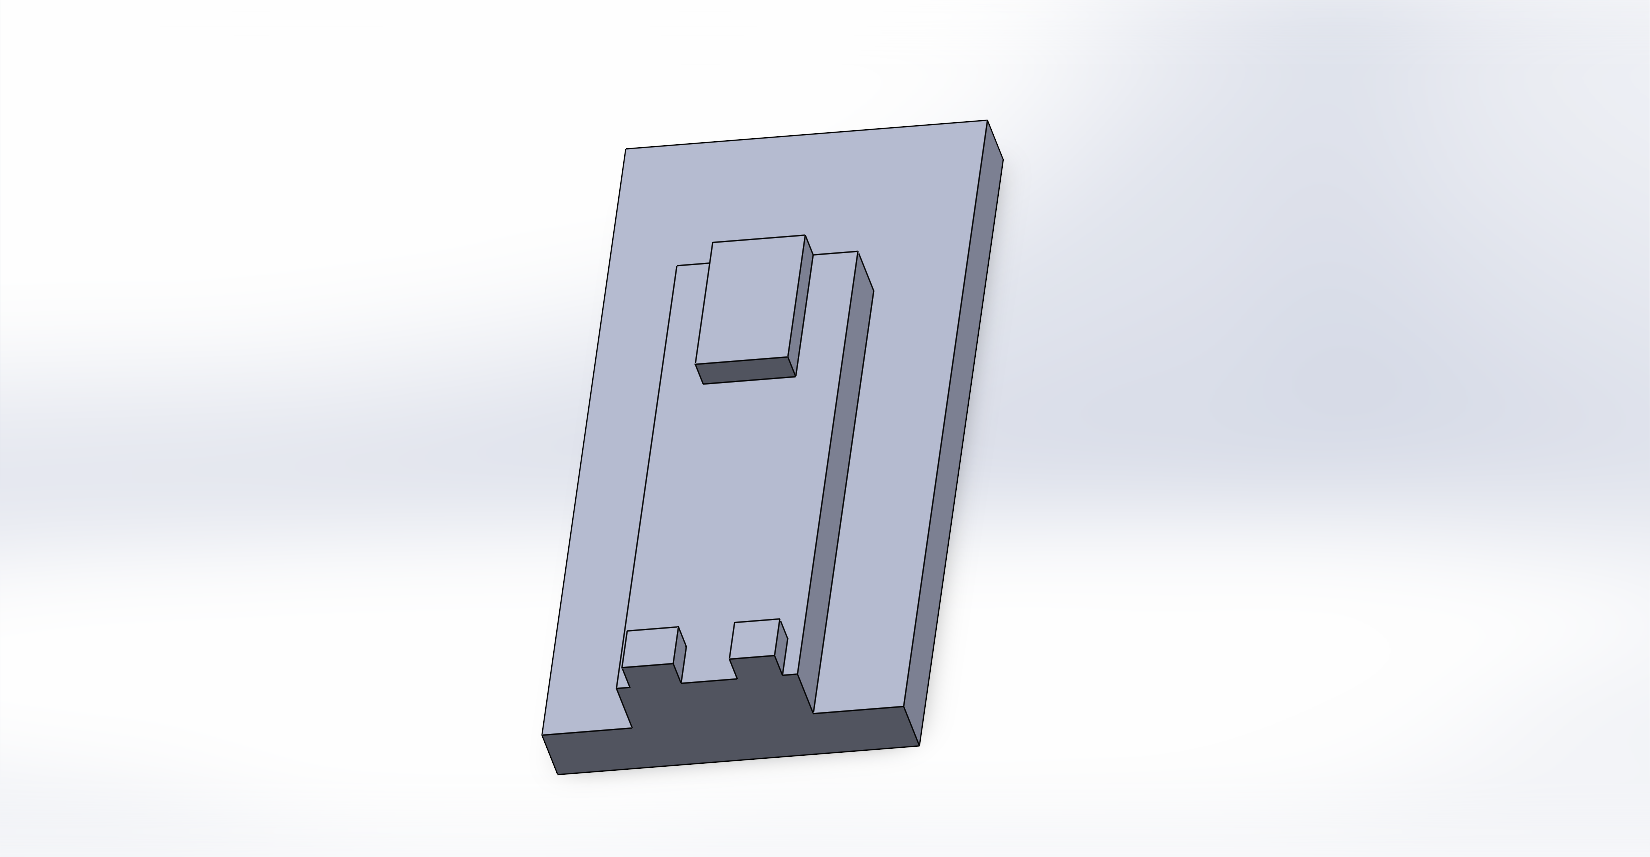
\includegraphics[height=19mm]{7/img/Piezauno.PNG}  & 
       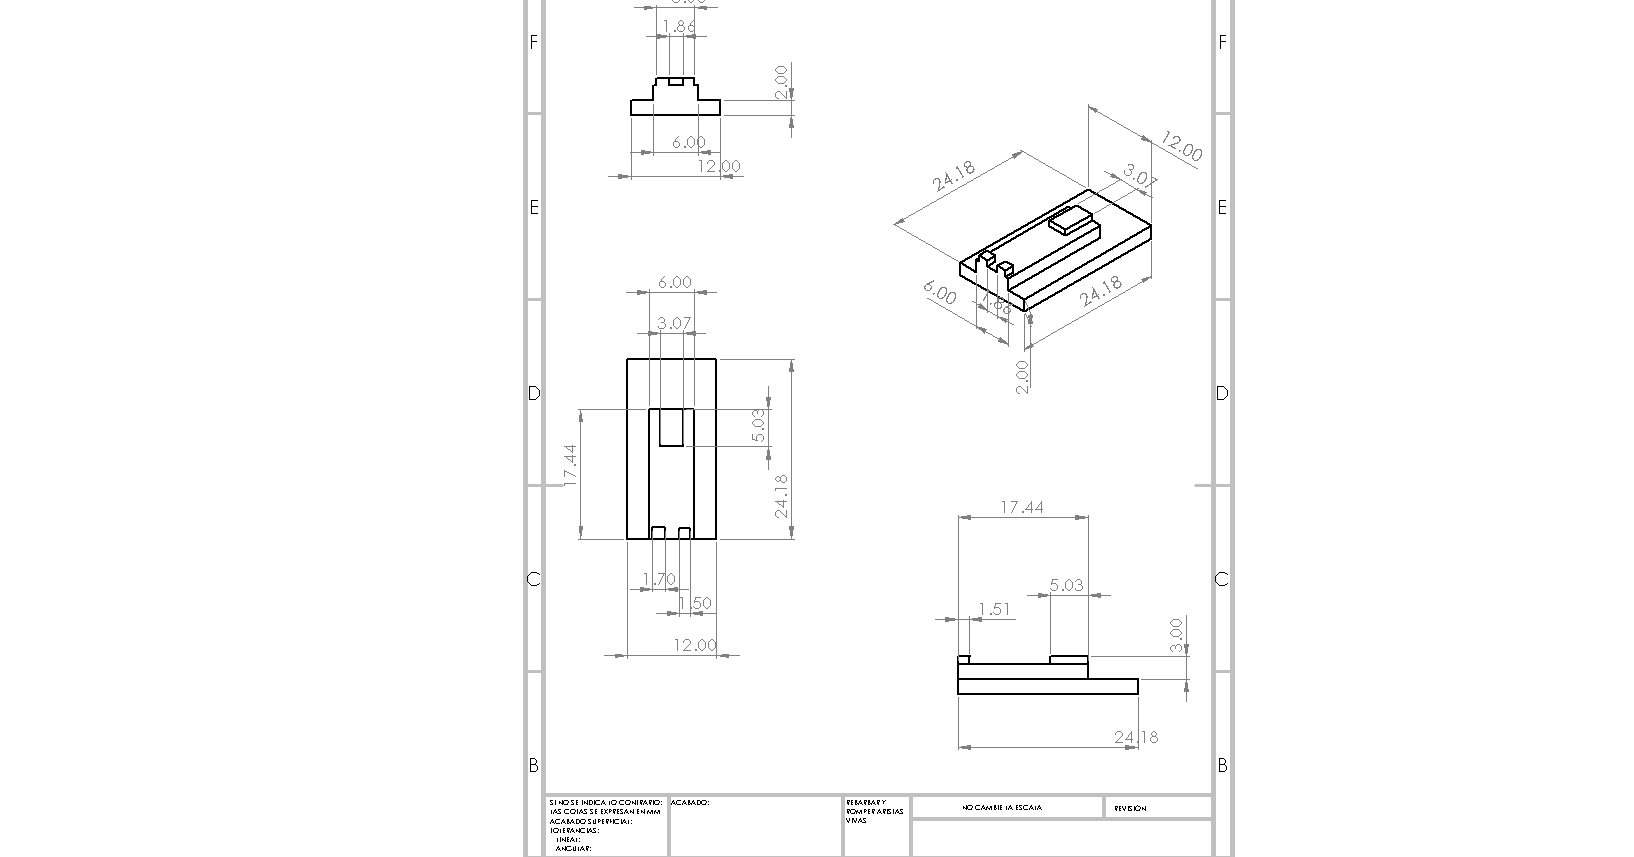
\includegraphics[width=19mm]{7/img/Pieza2.PNG}  \\
        \hline
        lcd & 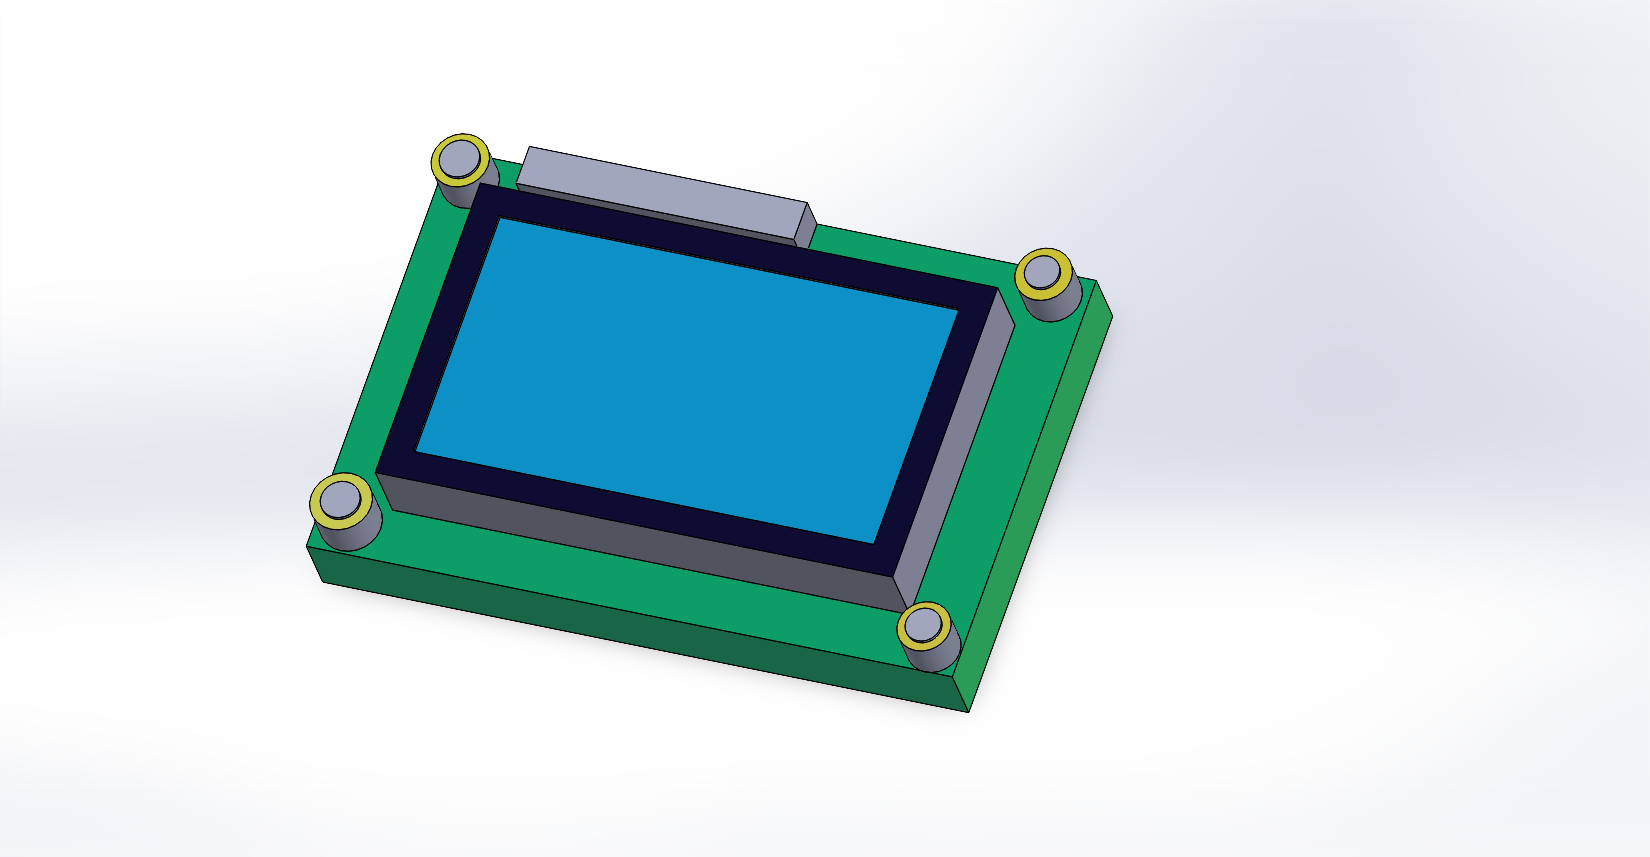
\includegraphics[height=19mm]{7/img/piezatress.PNG}  & 
       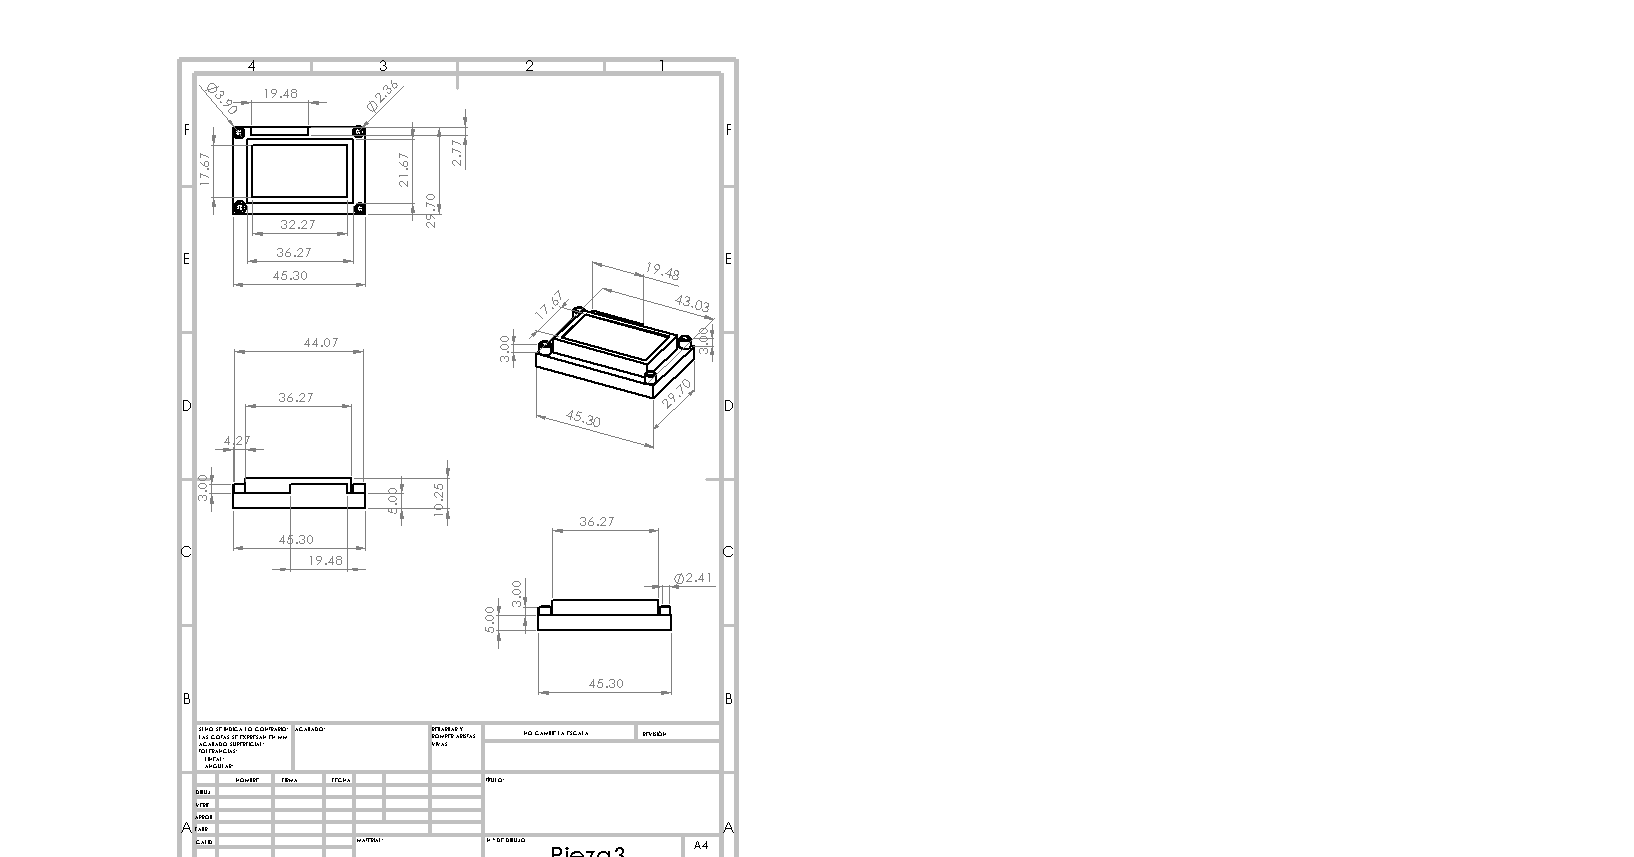
\includegraphics[width=19mm]{7/img/Pieza3.PNG} \\
        \hline
        cable HM & 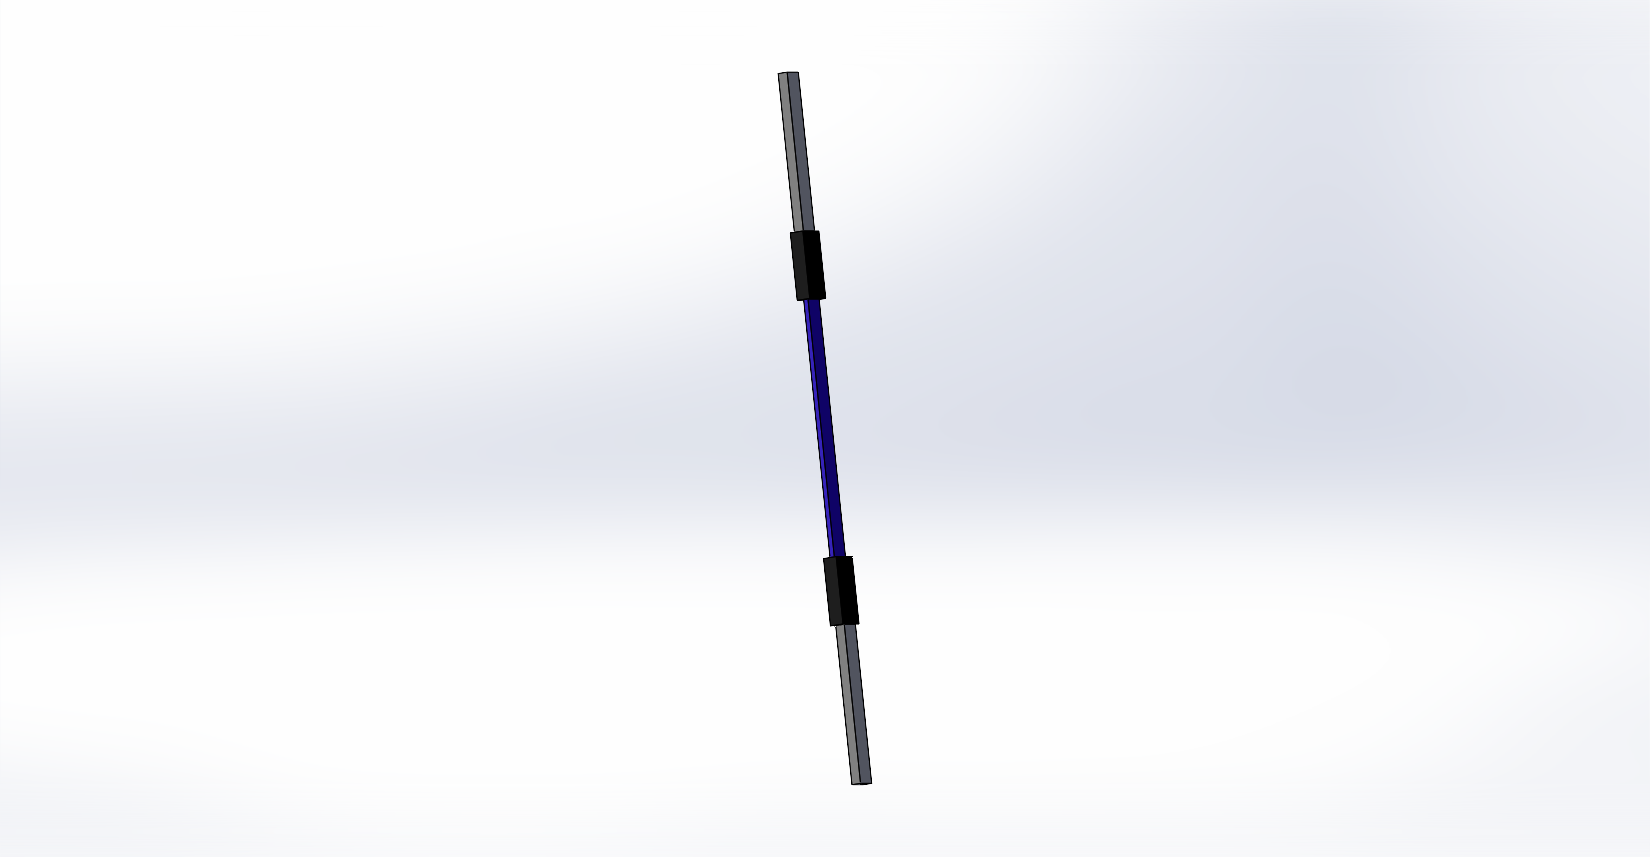
\includegraphics [height=19mm]{7/img/cuatrooo.PNG}  & 
       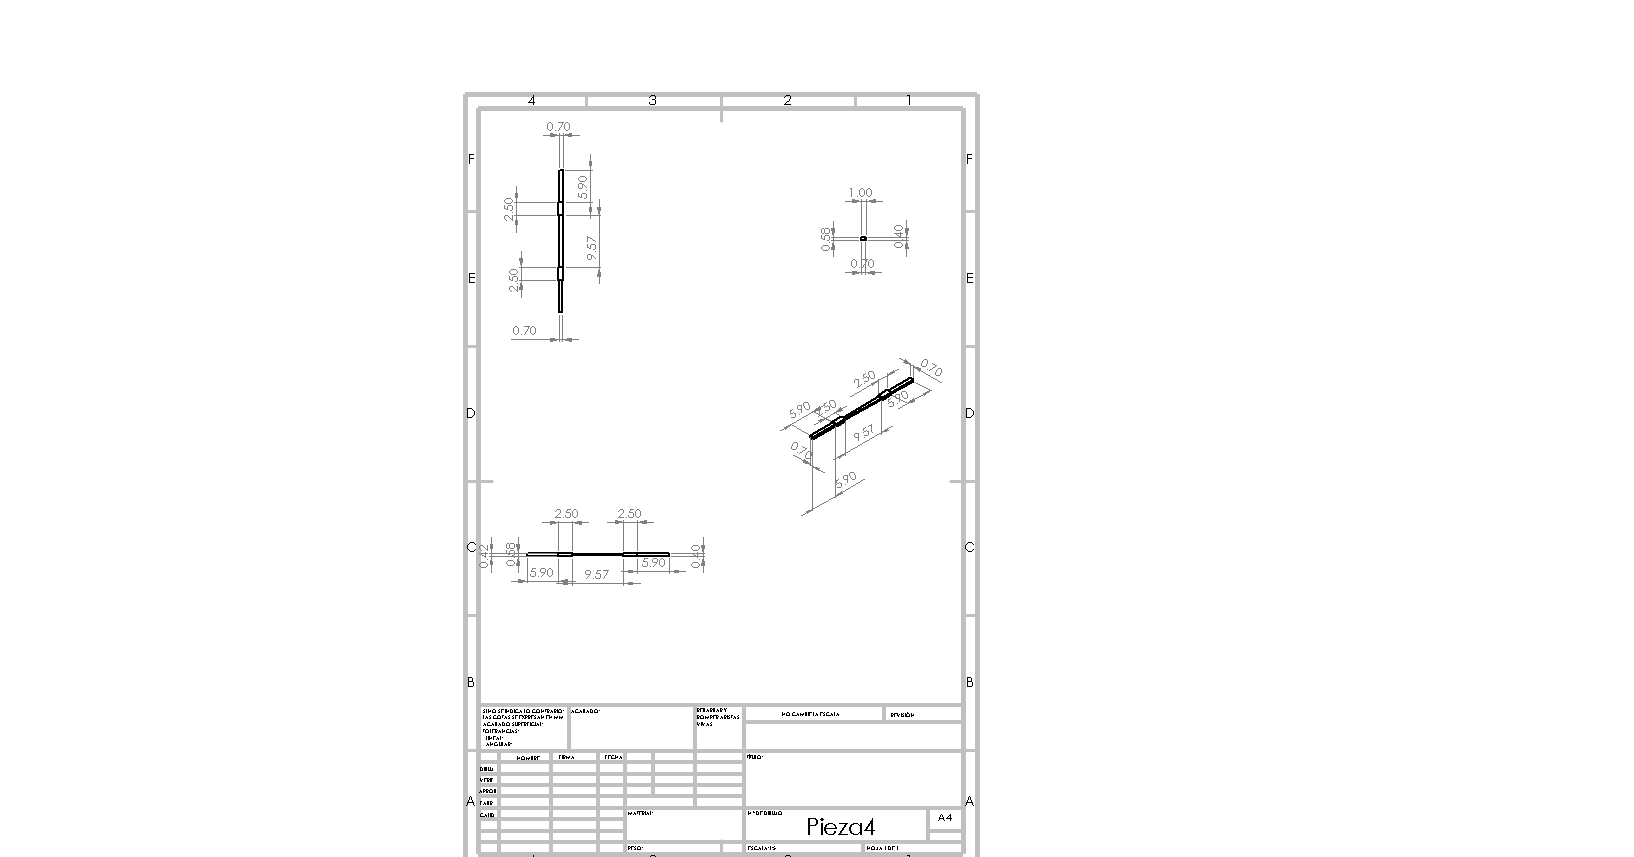
\includegraphics[width=19mm]{7/img/Pieza4.PNG} \\
        \hline
        CABLE HH & 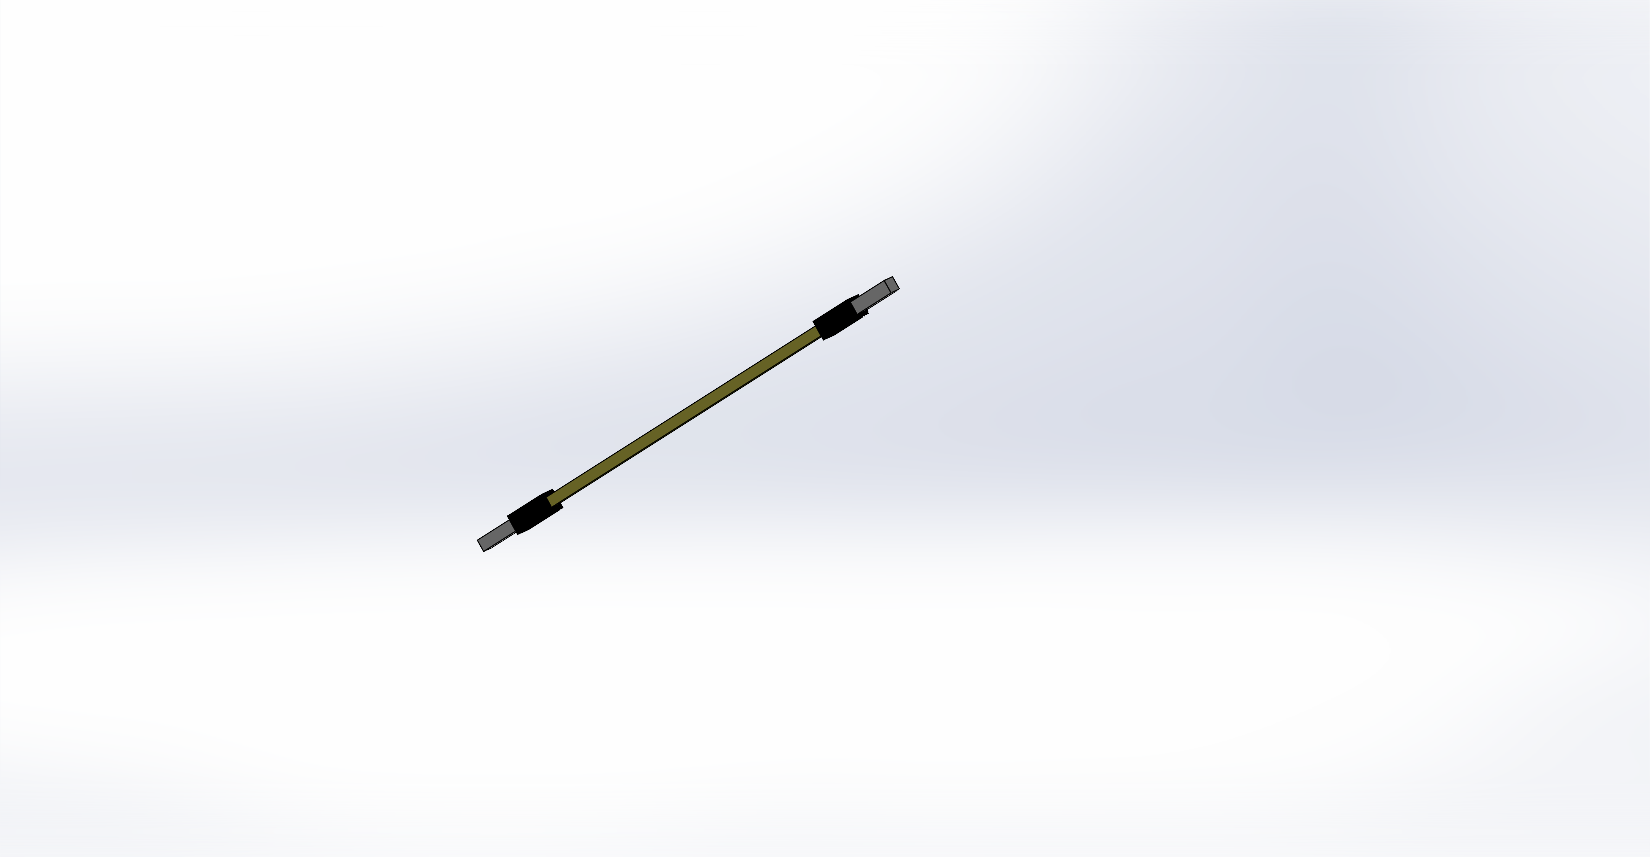
\includegraphics[height=19mm]{7/img/cinco.PNG}  & 
       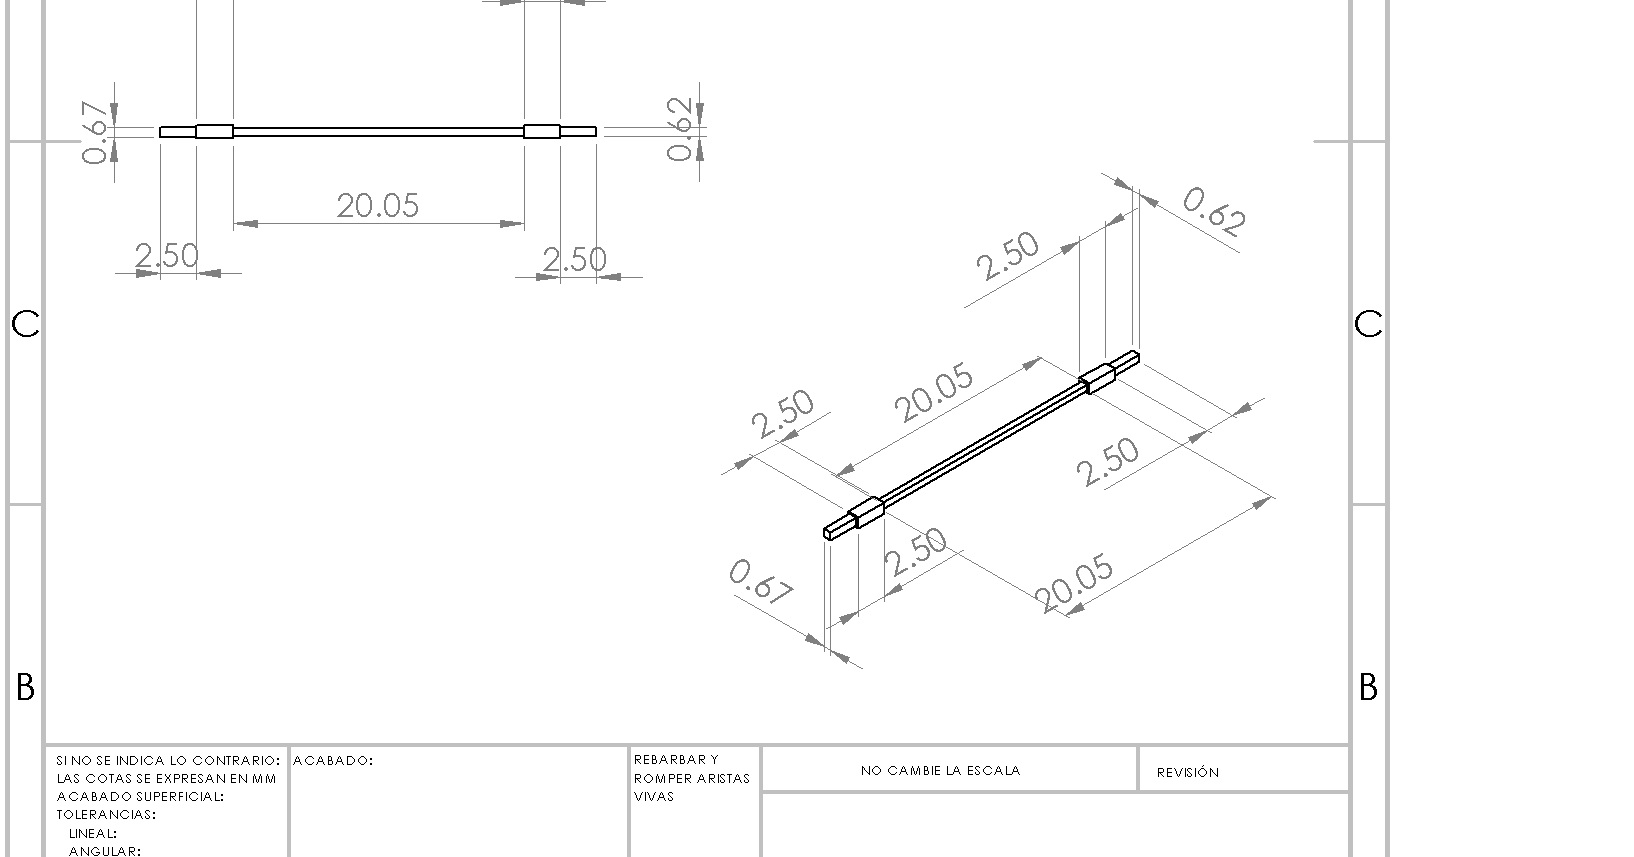
\includegraphics[width=19mm]{7/img/Pieza5.PNG} \\
        \hline 
         CABLE 1 & 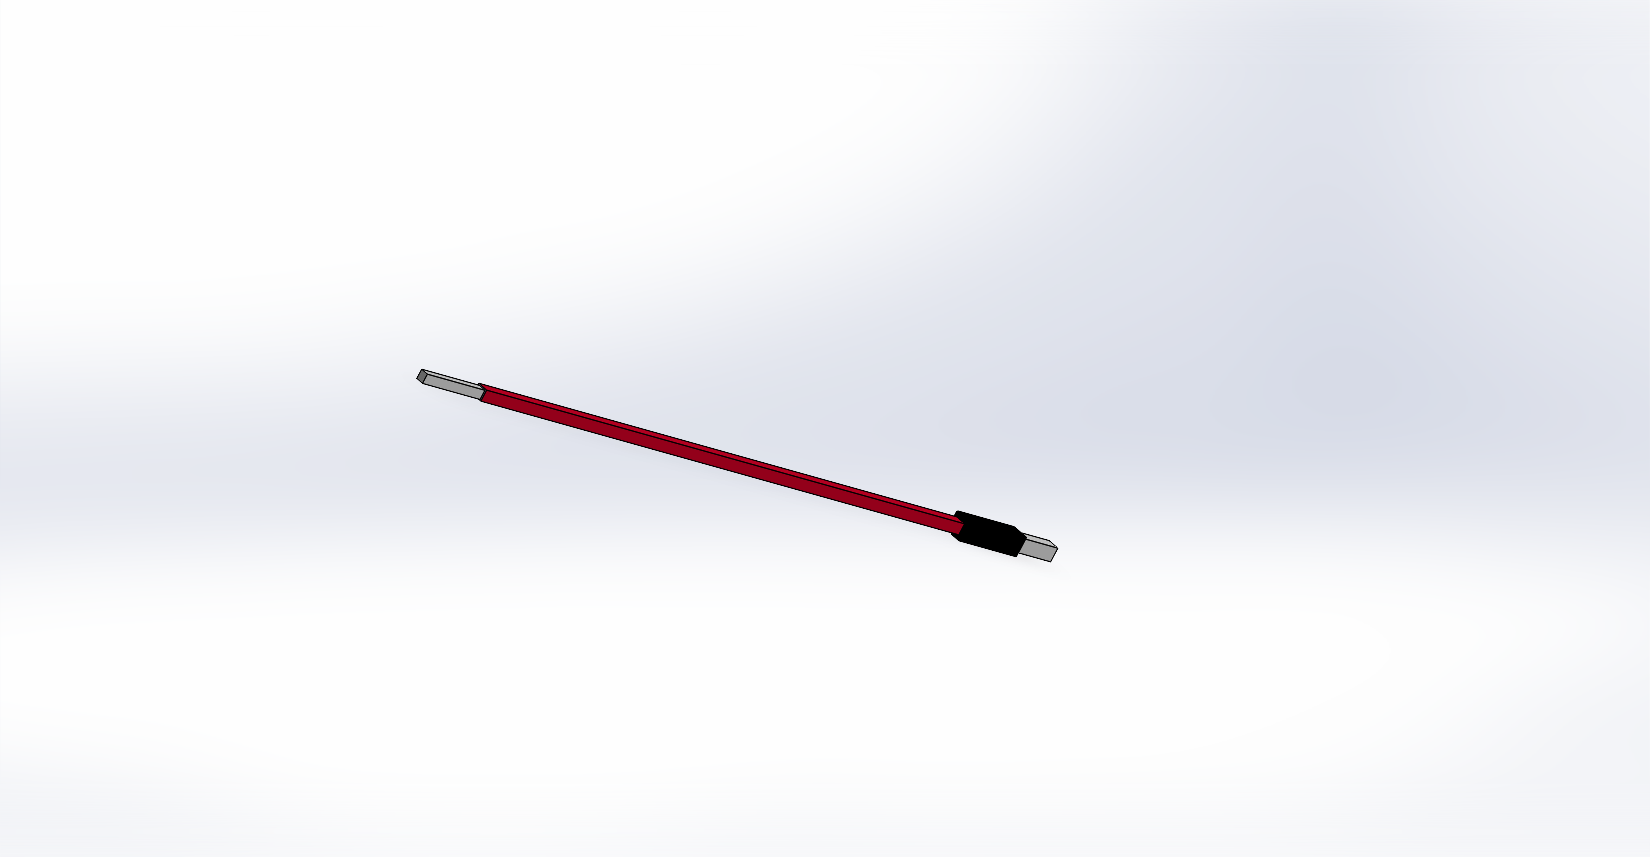
\includegraphics[height=19mm]{7/img/seis.PNG}  & 
       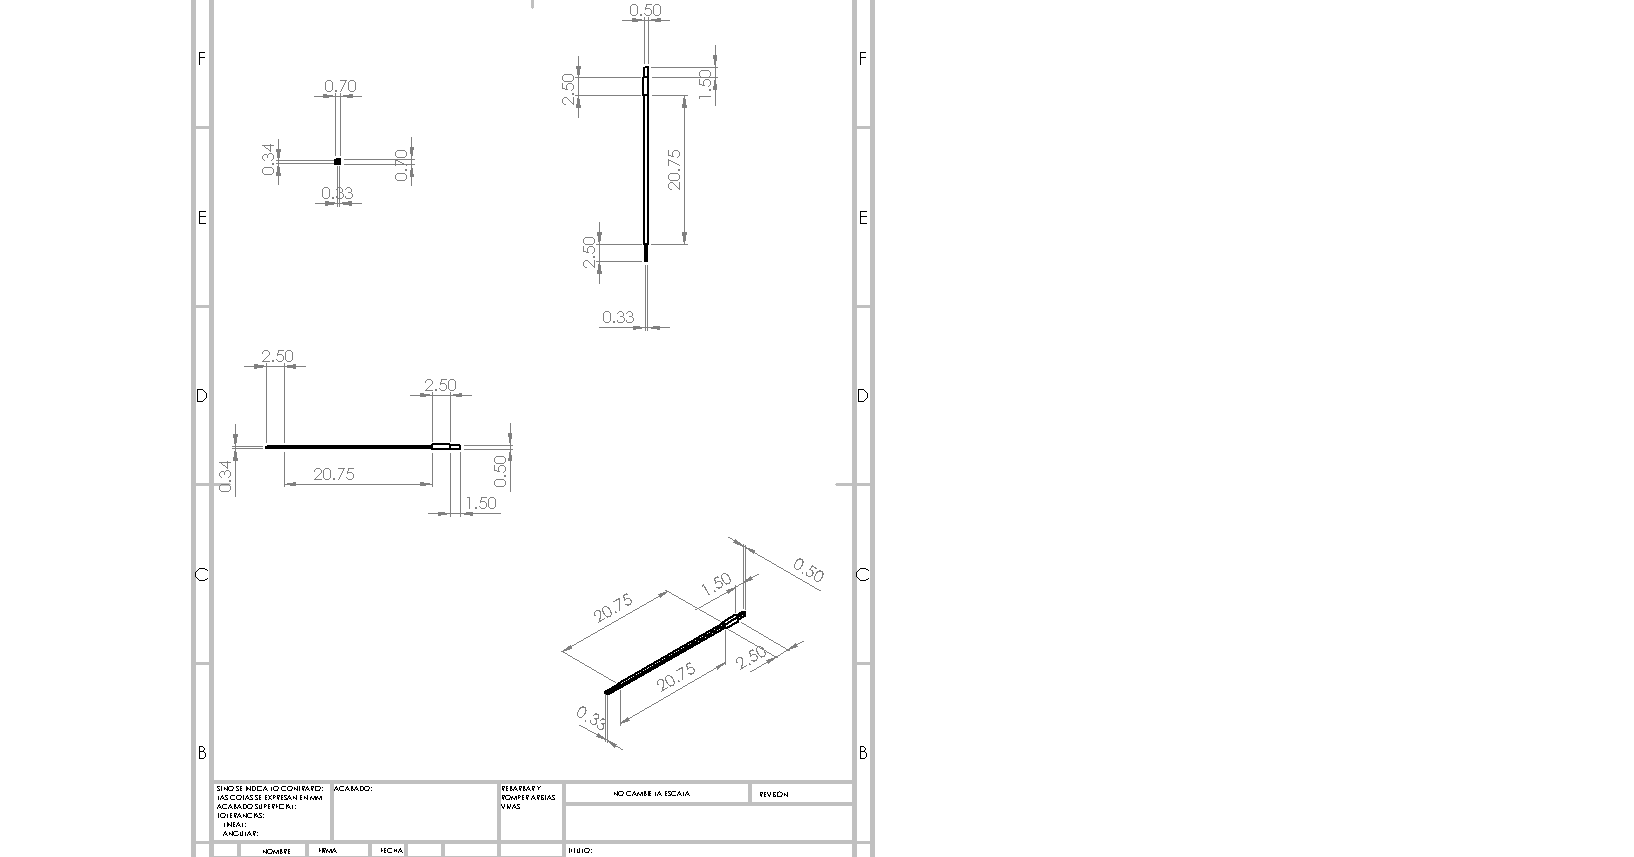
\includegraphics[width=19mm]{7/img/heymickey.PNG} \\
        \hline 
         CABLE 2 & 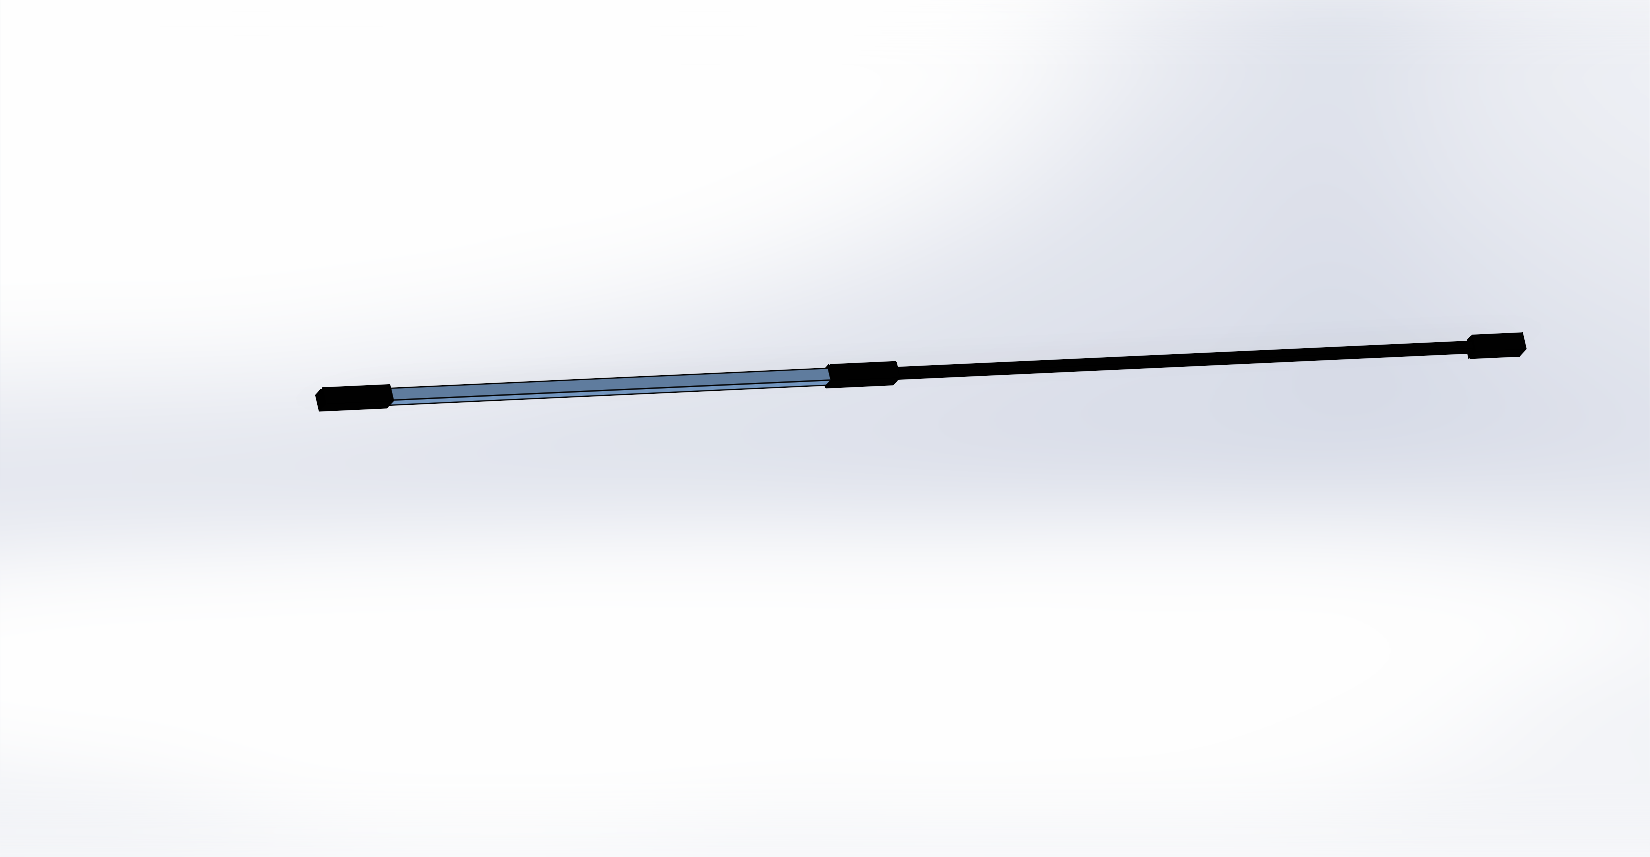
\includegraphics[height=19mm]{7/img/siete.PNG}  & 
       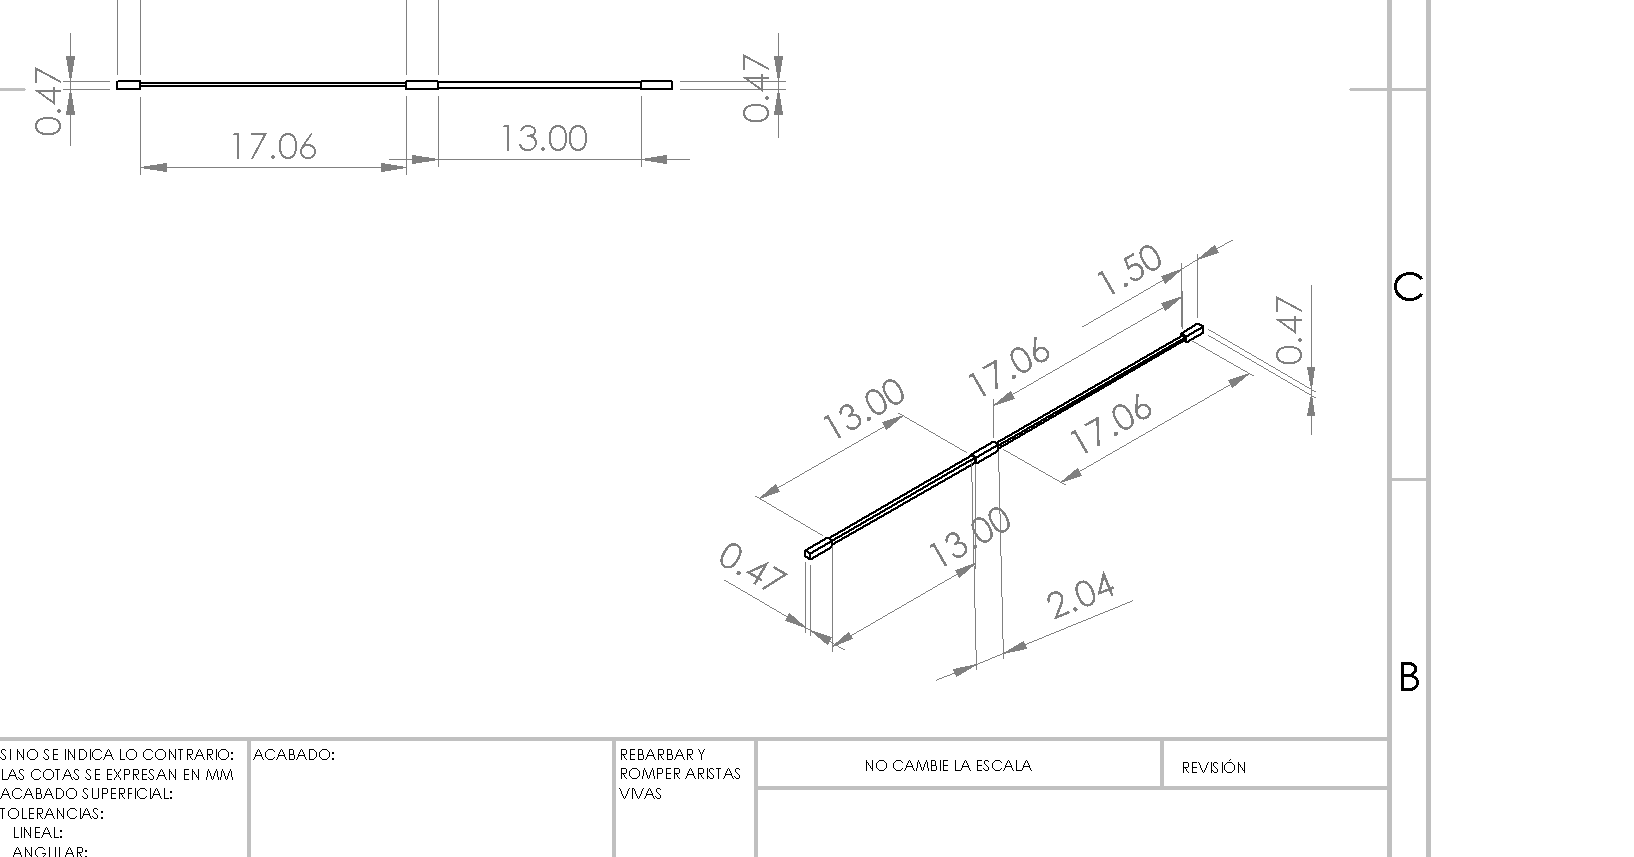
\includegraphics[width=19mm]{7/img/siu.PNG} \\
        \hline 
        
        \end{tabular} 
       
         \label {tab:my_label3}  \label {}
          \end{table} 
    
      \begin{tabular}{c|c}
           &  \\
           & 
      \end{tabular}  
    
    
    \section{Resultados y discusión}
    
    Como uno de los resultados y discusiones que se hizo durante todo este proyecto es que la importancia de ver y con llevar nuevos retos que estuvieron de otro nivel es importante para tu formacion como ingeniero ya que  siempre te vas a enfrentar a nuevos retos que a lo mejor no sabes o que si sabes pero lo importante es seguir y analizar cada proyecto que se presente. 
    
    El principal resultado fue logrado ya que se hizo de una manera correcta la implementacion de todas las figuras haciendo que su uso final nos indicara los niveles de voltaje de una mejor manera y que sobretodo funcionara ya que la principal discusion era el correcto manejo de como conectar y hacer bien los ensambles ya sea de los cables o del protoboard.  \newline
     \newline
    Al tener presente este tema pudimos seguir los pasos de una manera correcta y eficaz haciendo que el usuario comprendiera y entendiera el mejor manejo que se le pudo dar esto presento que al final el resultado fuera el obtenido y el que se esperaba desde un principio .  \newline
     \newline
    Cada una de las etapas es de suma importancia ya que esto sigue un proceso el cual se fue siguiendo paso a paso con sus debidas instrucciones para que se pudiera hacer el debido cumplimiento del proyecto .  \newline
     \newline
    
    
    
    \section{Conclusiones}
    
    Una de las principales conclusiones es que el proyecto fue de mucha retroalimentacion como ingeniero es que represento un nuevo reto para mi ya que me saco de mis casillas y me represento nuevas formas para poder retroalimentar mi conocimiento y como me fui desenvolviendo durante el transcurso del proyecto y esto significo un avance importante para mi. \newline
     \newline
     Esto significa que como ingeniero puede representar diferentes nuevos retos para que nosotros como personas tenemos que buscar diferentes alternativas y soluciones para proyectos o retos que no comprendamos y que necesitamos investigar para fortalecer el conocimiento y emplearlo de una mejor manera para que asi nosotros lo podamos cumplir de una buena forma.  \newline
      \newline
    Como conclusion general puedo decir que este proyecto me sirvio como persona ya que al principio no le tenia el minimo interes pero esto fue cambiando conforme fue avazando se me fue haciendo mas interesante ya que ver cada etapa de este proceso significo muy interesante para tener una idea de como seria un proyecto de residencia profesional y como ir afrontandolo poco a poco  \newline
    
    \section{Agradecimientos}
    
    Es importante darle su reconocimiento a las fuentes de informacion que me ayudaron y brindaron algunas ideas como lo son Google y la plataforma de Youtube esto haciendo incapie a la ayuda que me brindaron y esto haciendo que me ayudara un poco mejor el proceso de como fui llevando el proyecto , tambien quiero darle un agardecimiento a mis compañeros que me brindaron la ayuda de como manejar el proyecto y sobretodo un agradecimiento a mi profesor .
    
    \section*{Referencias}
    
    %Para esta platilla, se solicita al autor enumerar las citas de manera consecutiva entre corchetes \cite{YLi2013}. 
    %La puntuación de la oración que sigues sería \cite{Mesaelides2011}. 
    %Refiérase simplemente al número de referencia, como en \cite{Morales2012}, no utilice “Ref. [3]” o “referencia [3]” excepto al principio de una oración: “La referencia [3] fue la primera…”
    Enumere las notas al pie por separado en superíndices. Coloque la nota de pie de en la parte inferior de la columna en la que se citó. No coloque notas al pie en la lista de referencias. Utilice letras para las notas al pie de la tabla.
    A menos de que haya tres autores o más; no utilice “et al.”. Los trabajos que no hayan sido publicados, incluso si han sido presentados para su publicación, deben ser citados como “inéditos”. Los trabajos que han sido aceptados para su publicación deben de citarse como “en prensa”. Poner en mayúscula sólo la primera palabra de un título, excepto los nombres propios y los símbolos de elemento. 
    
    %Otros ejemplos \cite{LAAngeles2021}, \cite{LAAngelesConni}. 
    
    % Ejemplo
    %  @Article{article,
    % 	author = "Author1 LastName1 and Author2 LastName2 and Author3 LastName3",
    % 	title = "Article Title",
    % 	volume = "30",
    % 	number = "30",
    % 	pages = "10127-10134",
    % 	year = "2013",
    % 	doi = "10.3389/fnins.2013.12345",
    % 	URL = "http://www.frontiersin.org/Journal/10.3389/fnins.2013.12345/abstract",
    % 	journal = "Frontiers in Neuroscience"
    % }
    
    % @book{book,
    %   author    = {Author Name}, 
    %   title     = {The title of the work},
    %   publisher = {The name of the publisher},
    %   address   = {The city},
    %   year      = 1993,
    % }
    
    % @incollection{chapter,
    %   author       = {Bauthor Surname}, 
    %   title        = {The title of the work},
    %   editor       = {Editor Name},
    %   booktitle    = {The title of the book},
    %   publisher    = {The name of the publisher},
    %   address      = {The city},
    %   year         = 2002,
    %   pages        = {201-213},
    % }
    
    % @InProceedings{conference,
    %   author = {Cauthor Name and Dauthor Surname and Fauthor LastName},
    %   title = {The title of the work},
    %   booktitle = {The title of the conference proceedings},
    %   year = 1996,
    %   publisher = {The name of the publisher},
    %   editor = {Editor Name1 and Editor Name2},
    %   pages = {41-50},
    % }
    
    % @book{cho,
    %   author       = {Gauthor Name1}, 
    %   title        = {The title of the work},
    %   publisher = {Country code and patent number},
    %   address      = {Patent Country},
    %   year = 2013
    % }
    
    % @book{patent,
    %   author    = {Hauthor Surname1}, 
    %   title     = {The title of the work},
    %   publisher = {Patent number},
    %   address   = {Patent country},
    %   year      = 2010,
    % }
    
    % % please use misc for datasets
    % @misc{dataset, 
    % 	author = "Author1 LastName1 and Author2 LastName2 and Author3 LastName3",
    % 	title = "Data Title",
    % 	year = "2011",
    % 	doi = "10.000/55555",
    % 	URL = "http://www.frontiersin.org/",
    % }
    
    \bibliographystyle{ieeetr}
    \bibliography{7/referencias} 